\pagestyle{empty}
\cleardoublepage
\pagestyle{fancy}
\chapter{Teste e Validação dos Modelos}\label{cap3}

\section{Resultados e Discussão $\cdot$ Matriz $M$}\label{cap3:ModelM}

\subsection{Seleção Estabilizadora}

Para implementar o modelo com matriz $M$ inicialmente procuramos
reproduzir os resultados obtidos em \cite{Jones2007}, focando no
alinhamento entre matriz G e matriz $\omega$ pela seleção indireta na
matriz $M$. 
Esse efeito pode ser observado na figura \ref{jones2tracos}, onde vemos
a correlação entre dois traços aumentando em resposta à atuação da
seleção estabilizadora correlacionada.  

\begin{center}
\begin{figure}[htbp]
  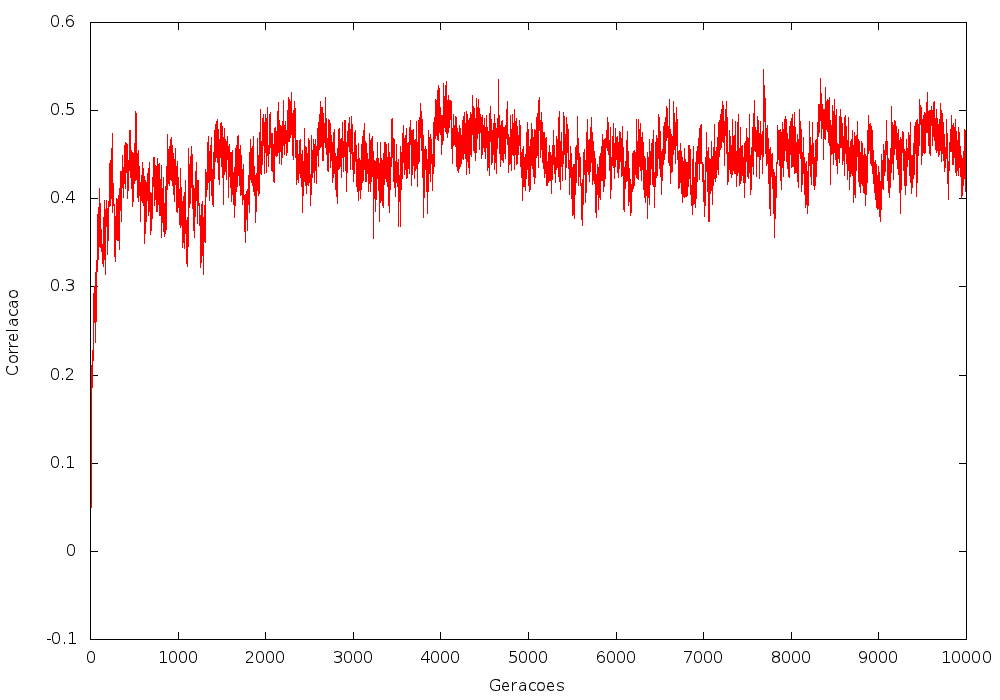
\includegraphics[width=150mm, height=80mm]{figuras/jones2tracos.png}
  \caption{Evolução da correlação entre dois traços ligados por efeitos
  mutacionais pleiotrópicos sobre seleção estabilizadora correlacionada.
  Nesta simulação $r_\omega=0.8$, $Ne=5000$, $p=2$, $m=50$}
  \label{jones2tracos}
\end{figure}
\end{center}

Como nosso objetivo é expandir a modelagem para mais traços, em seguida
adicionamos um traço ao sistema. 
Nesse caso, as considerações sobre a dificuldade de manter a matriz $M$
positiva definida já se aplicam, sendo necessário fazer uso da correção
de auto-valores. 
Mesmo assim, o resultado é bastante semelhante, ainda com a correlação
entre os 3 traços se alinhando com a matriz $\omega$ (figuras
\ref{jones3tracos} e \ref{MatJones3tracos}). 


\begin{center}
\begin{figure}[htbp]
  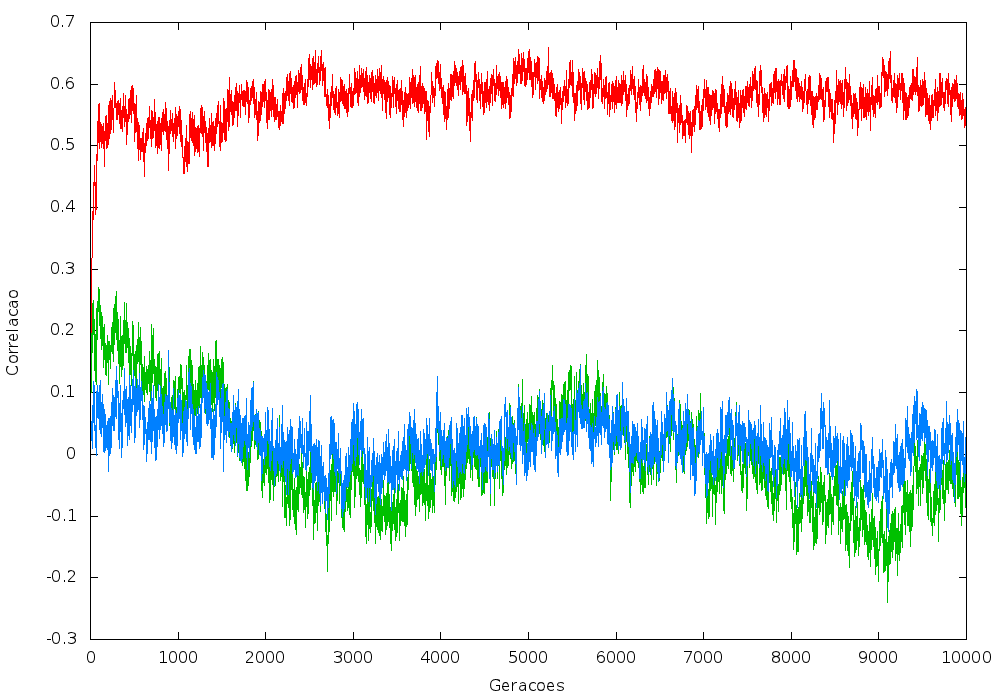
\includegraphics[width=150mm, height=80mm]{figuras/jones3tracos.png}
  \caption{Evolução da correlação entre três traços ligados por efeitos
  mutacionais pleiotrópicos sobre seleção estabilizadora correlacionada.
  A seleção propicia a integração entre dois traços (linha vermelha) e a desistegração
  desses dois com o terceiro (linhas azul e verde). Nesta simulação
  $r_\omega$ como na equação \ref{romega}, $Ne=5000$, $p=3$, $m=50$.}
  \label{jones3tracos}
\end{figure}
\end{center}

Na figura \ref{MatJones3tracos} vemos representações gráficas da matriz
de correlação fenotípica ao final da simulação e da matriz $\omega$ de
seleção estabilizadora correlacionada. 
Caselas mais claras indicam correlação maior. 
Nesse caso a matriz de correlação mutacional usada foi:

\begin{equation}
Corr(\omega) = \left( \begin{smallmatrix} 1 & 0.9 & 0.1\\  0.9 & 1 & 0.1 \\ 0.1 & 0.1 & 1 \end{smallmatrix}  \right)
\label{romega}
\end{equation}

E a matriz de covariância mutacional: 

\begin{equation}
\omega = \left( \begin{smallmatrix} 9 & 8.1 & 0.9\\  8.1 & 9 & 0.9 \\ 0.9 & 0.9 & 9 \end{smallmatrix}  \right)
\end{equation}

\begin{center}
\begin{figure}[htbp]
  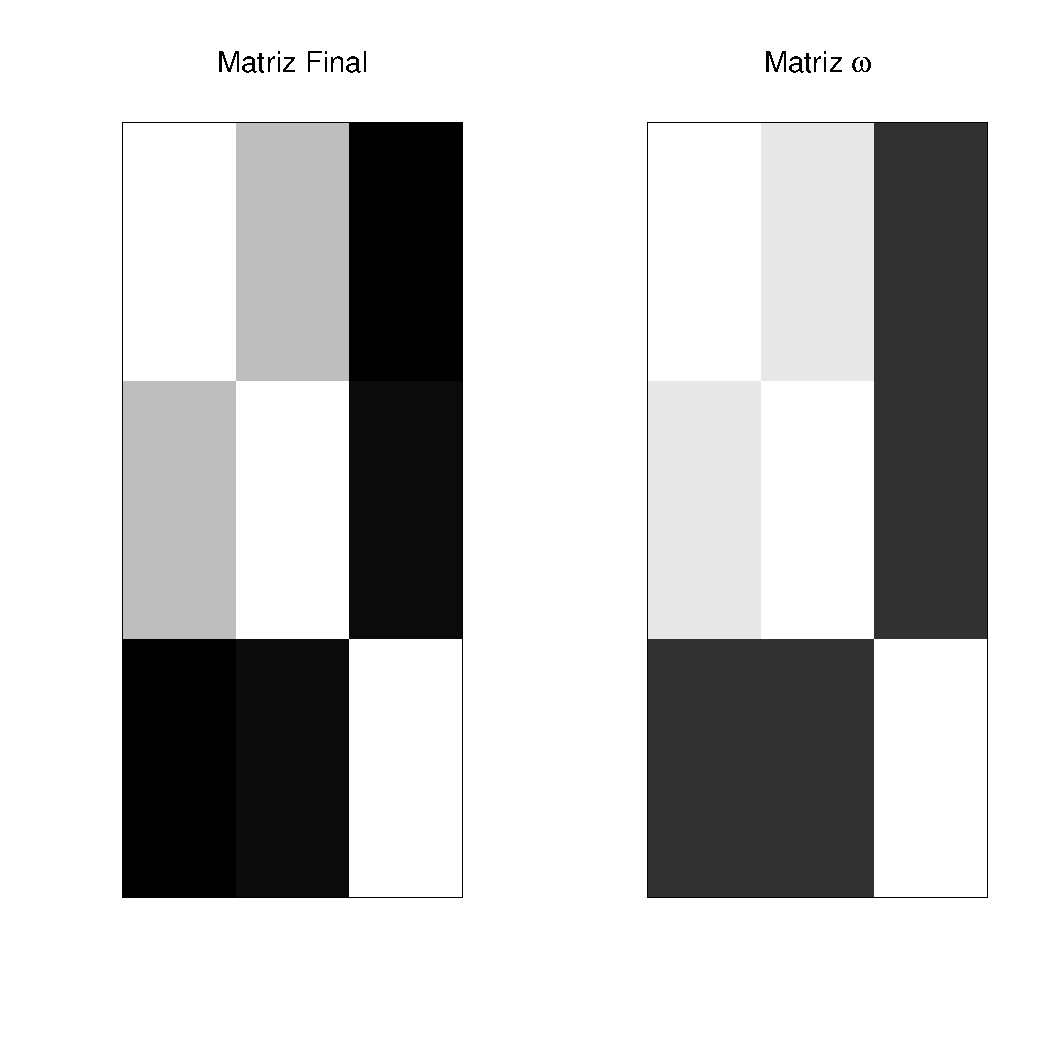
\includegraphics[width=150mm, height=80mm]{figuras/Mat3tracos}
   \caption{Comparação entre a matriz de correlação final para o 3
   traços após 10000
   gerações de seleção e a matriz $\omega$ da superfície de seleção.}
  \label{MatJones3tracos}
\end{figure}
\end{center}

Quando procuramos ampliar o número de traços, porém, o alinhamento da
matriz G com a matriz $\omega$ se mostrou problemático. 
Nesse caso a matriz de correlação da superfície de seleção continha dois
módulos, e era dada por:

\begin{equation}
Corr(\omega) = \left( 
\begin{smallmatrix} 
1 & 0.8 & 0.8 & 0.8 & 0.8 & 0 & 0 & 0 & 0 & 0\\  
0.8 & 1 & 0.8 & 0.8 & 0.8 & 0 & 0 & 0 & 0 & 0\\  
0.8 & 0.8 & 1 & 0.8 & 0.8 & 0 & 0 & 0 & 0 & 0\\  
0.8 & 0.8 & 0.8 & 1 & 0.8 & 0 & 0 & 0 & 0 & 0\\  
0.8 & 0.8 & 0.8 & 0.8 & 1 & 0 & 0 & 0 & 0 & 0\\  
0 & 0 & 0 & 0 & 0 & 1 & 0.8 & 0.8 & 0.8 & 0.8\\ 
0 & 0 & 0 & 0 & 0 & 0.8 & 1 & 0.8 & 0.8 & 0.8\\
0 & 0 & 0 & 0 & 0 & 0.8 & 0.8 & 1 & 0.8 & 0.8\\
0 & 0 & 0 & 0 & 0 & 0.8 & 0.8 & 0.8 & 1 & 0.8\\
0 & 0 & 0 & 0 & 0 & 0.8 & 0.8 & 0.8 & 0.8 & 1
\end{smallmatrix}  \right)
\label{matw}
\end{equation}

Na figura \ref{jones10tracos} vemos a trajetória típica das correlações
fenotípicas com uma matriz $\omega$ com dois módulos (ver figura
\ref{MatJones10tracos}).  
Aqui não existe mais a distinção entre
correlações dentro de módulos (altas) e entre módulos (baixas). 
Os resultados da evolução da modularidade $L$ e do AVGRatio confirmam a
ausência de modularização do sistema. 
A modularidade $L$ apresenta uma leve subida ao longo da simulação, mas
o AVG-Ratio permanece estável (Figura \ref{jones10tracosStats}). 
Isso se deve à modularidade $L$ capturar qualquer tipo de modularidade
na matriz, não só aquela associada a superfície de seleção. 
Na figura \ref{MatJones10tracos} fica claro que não existe semelhança
entre as matrizes G e $\omega$. 
Realizamos essas simulações com uma gama grande de intensidades de
seleção e chegando até 100000 gerações de seleção, sem nenhum indício de
alinhamento entre as matrizes $\omega$ e G.  

\begin{center}
\begin{figure}[htbp]
  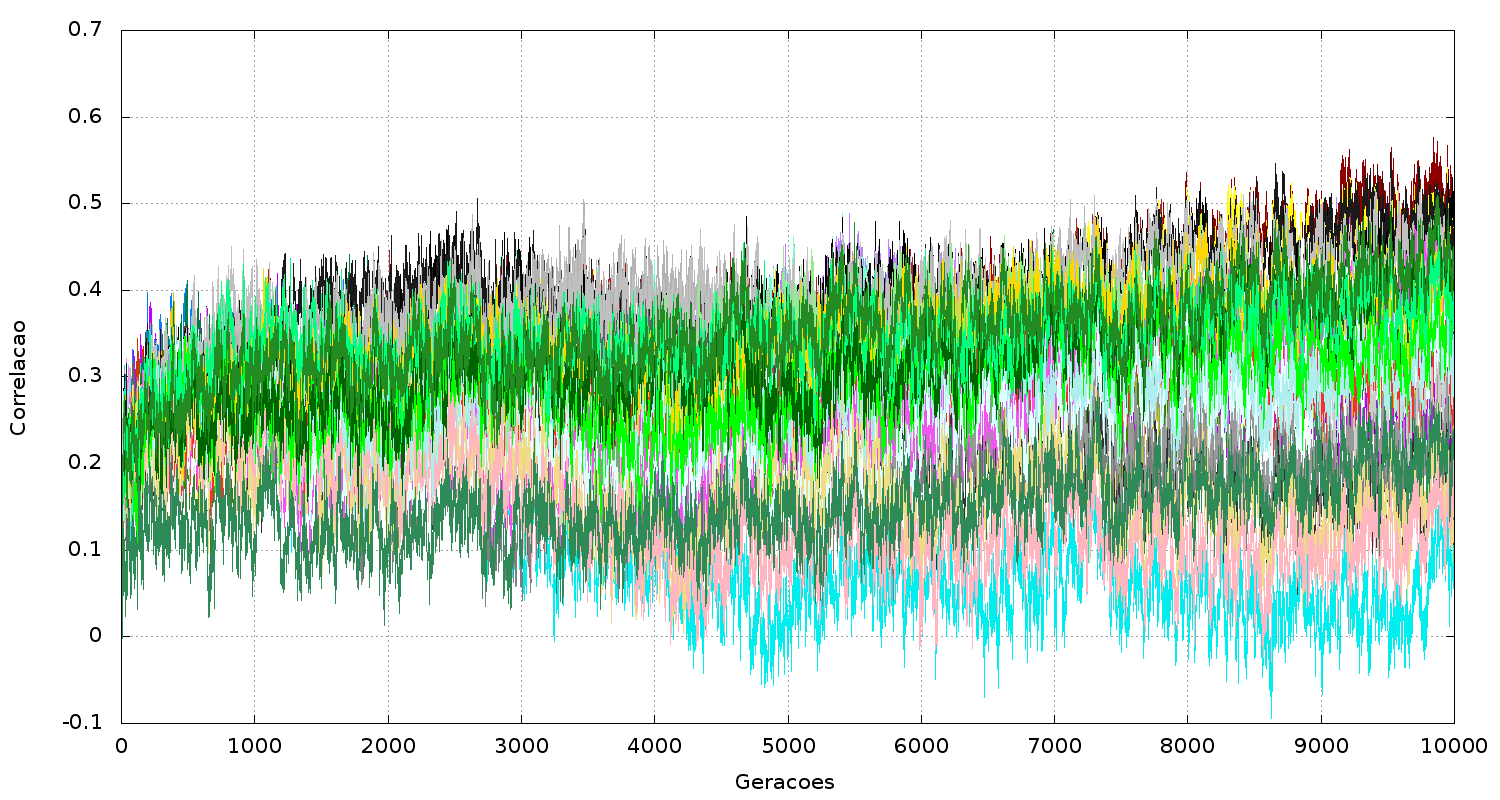
\includegraphics[width=150mm, height=80mm]{figuras/jones10tracos.png}
  \caption{Evolução da correlação entre dez traços ligados por efeitos
  mutacionais pleiotrópicos sobre seleção estabilizadora
  correlacionada. Apesar de a seleção promover a integração entre os
  5 primeiros e os 5 últimos traços e a desintegração entre esse
  módulos, isso não se transmite à matriz de correlação. Nesta simulação
  $r_\omega$ como na equação \ref{matw}, $Ne=5000$, $p=10$, $m=50$.}
  \label{jones10tracos}
\end{figure}
\end{center}

\begin{center}
\begin{figure}[htbp]
  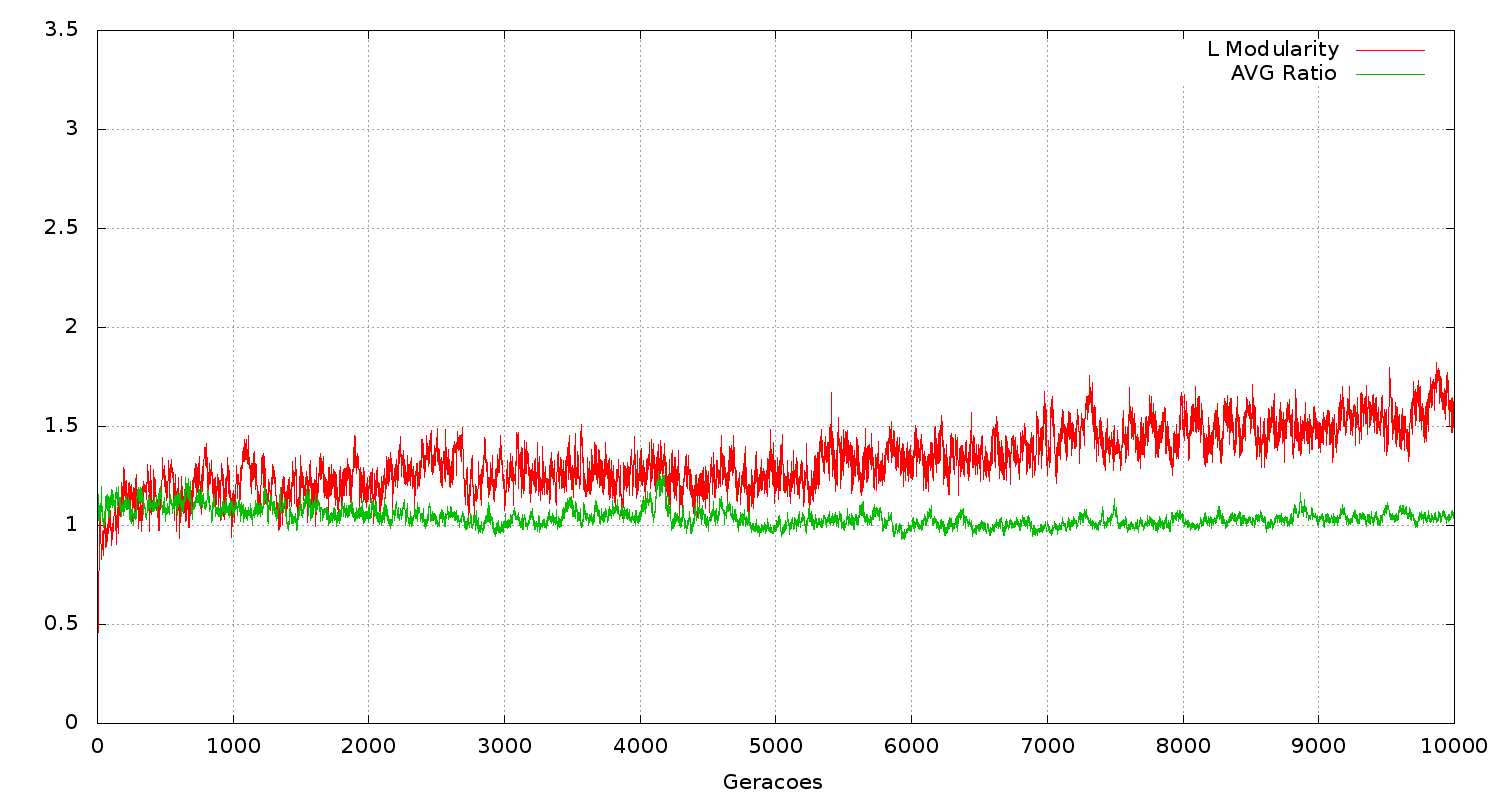
\includegraphics[width=150mm, height=80mm]{figuras/jones10tracosStats.png}
  \caption{Evolução da modularidade $L$ e AVG-Ratio para as matrizes de
  correlação representadas na figura \ref{jones10tracos}}
  \label{jones10tracosStats}
\end{figure}
\end{center}

\begin{center}
\begin{figure}[htbp]
  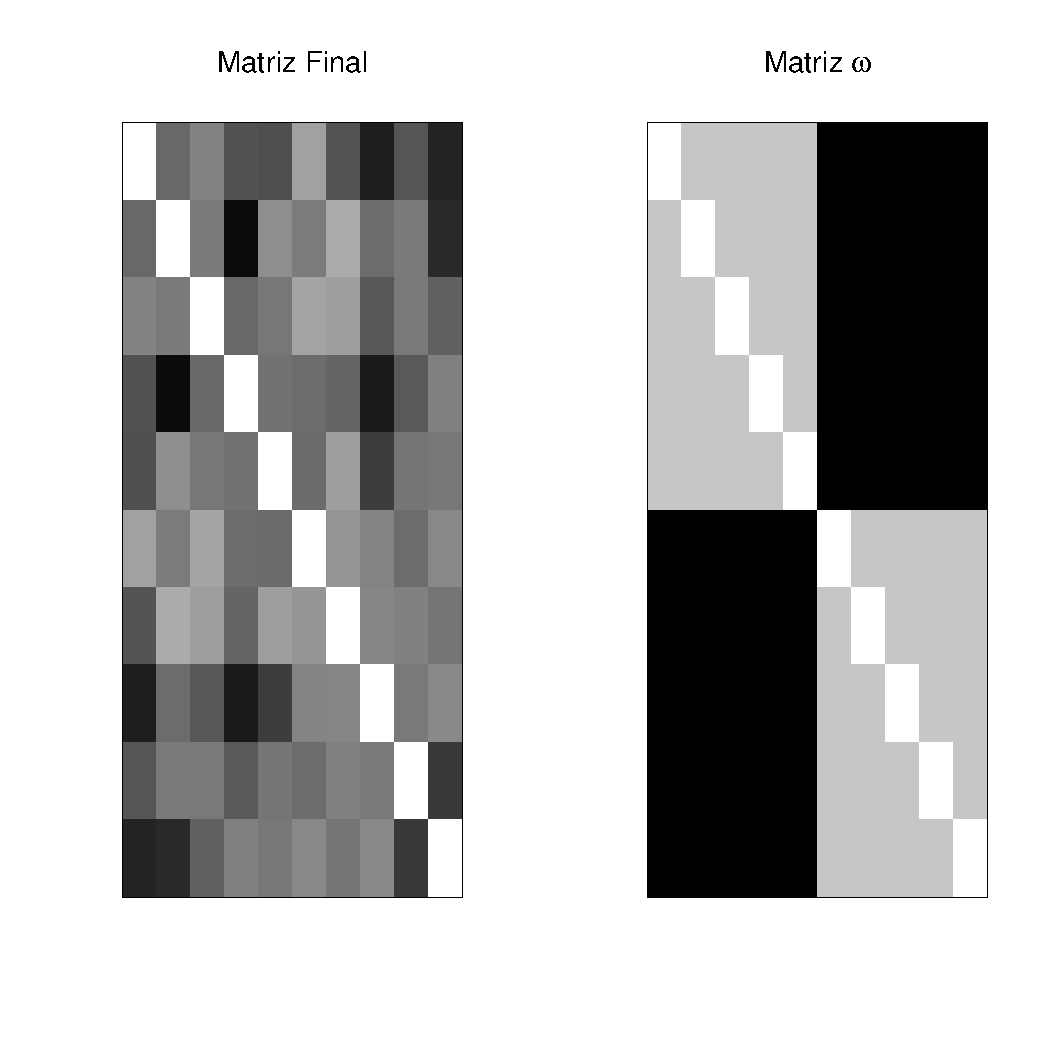
\includegraphics[width=150mm, height=80mm]{figuras/Mat10tracos}
  \caption{Comparação entre a matriz de correlação final para o 10
  traços após 10000 gerações de seleção representadas na figura
  \ref{jones10tracos} e a matriz $\omega$ da superfície de seleção.}
  \label{MatJones10tracos}
\end{figure}
\end{center}


\subsection{Seleção Direcional}

Em seguida, procuramos explorar como a inclusão de seleção direcional afetaria o
alinhamento das matrizes G e $\omega$. 
Utilizamos novamente uma matriz $\omega$ modular e acresentamos seleção
direcional correlacionada, de mudança conjunta na média dos traços
dentro de cada um dos módulos, e mudanças antagônicas entre módulos. 
Ou seja, os 5 primeiros traços tiveram seu ótimo fenotípico aumentado a
uma taxa constante e os 5 últimos traços tiveram seu ótimo reduzido de
forma simétrica ($\Delta_S=0.2$). 
As populações respondem a essa seleção de forma satisfátoria, alterando
suas médias de acordo com a posição do ótimo. 
Após 10000 gerações de seleção direcional, nós observamos a matriz final
e a evolução de todas as correlações genéticas nesse período. 
Os resultados podem ser vistos nas figuras \ref{jones10tracosDirecional}
, \ref{jones10tracosDirecionalStats} e \ref{MatJones10tracosDirecional}. 
Mesmo nessas condições, não observamos a emergência de módulos
variacionais na matriz G, que indicaria semelhança com a matriz $\omega$
e o padrão de seleção direcional correlacionada. 

\begin{center}
\begin{figure}[htbp]
  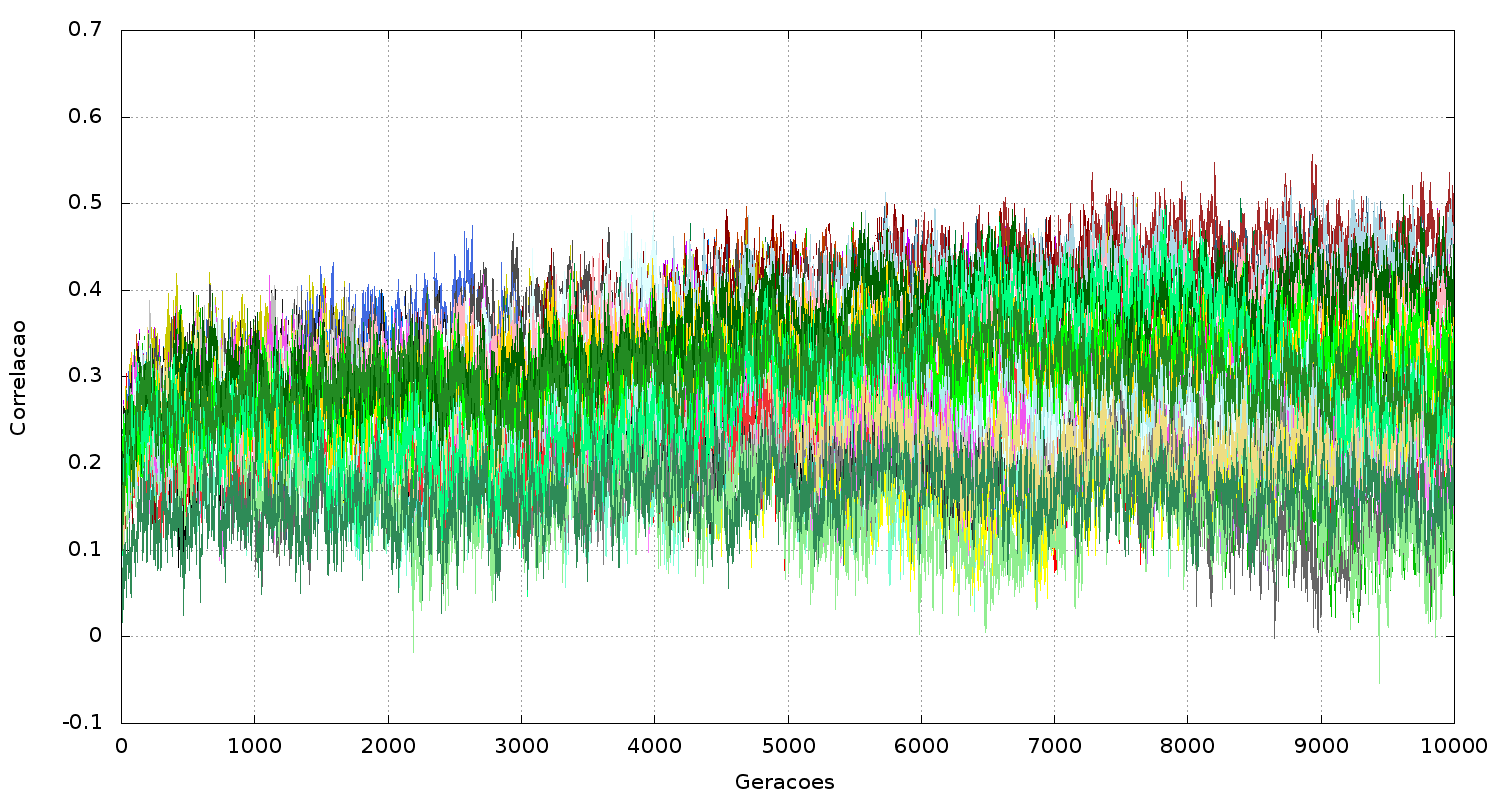
\includegraphics[width=150mm, height=80mm]{figuras/jones10tracosDirecional.png}
  \caption{Evolução da correlação entre dez traços ligados por efeitos
  mutacionais pleiotrópicos sobre seleção estabilizadora correlacionada
  e seleção direcional intensa para mudança correlacionada dentros dos
  módulos. Novamente, isso não se traduz na matriz de correlação genética.}
  \label{jones10tracosDirecional}
\end{figure}
\end{center}

\begin{center}
\begin{figure}[htbp]
  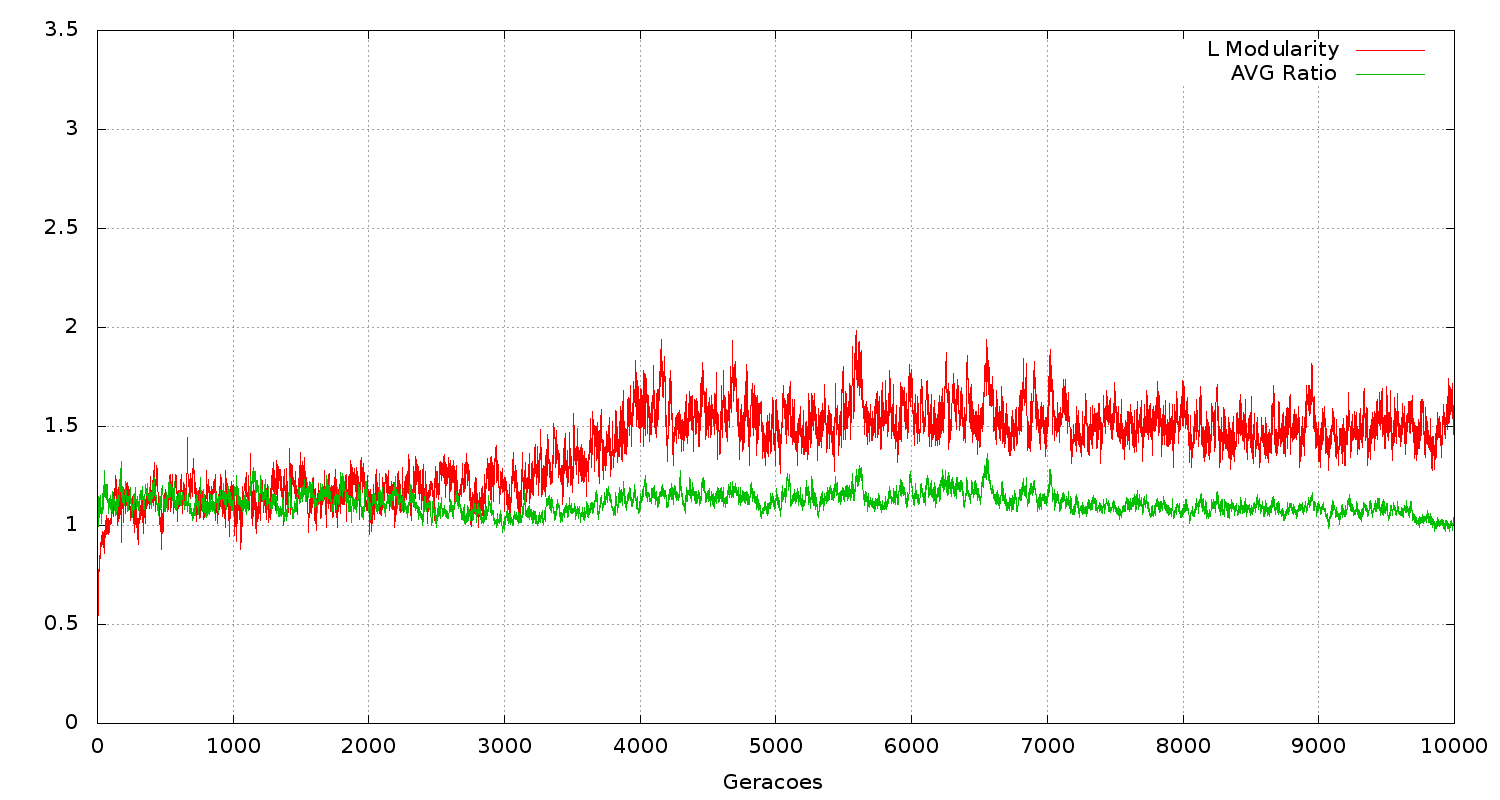
\includegraphics[width=150mm, height=80mm]{figuras/jones10tracosDirecionalStats.png}
  \caption{Evolução da modularidade $L$ e AVG-Ratio para as matrizes de
  correlação representadas na figura \ref{jones10tracosDirecional}}
  \label{jones10tracosDirecionalStats}
\end{figure}
\end{center}

\begin{center}
\begin{figure}[htbp]
  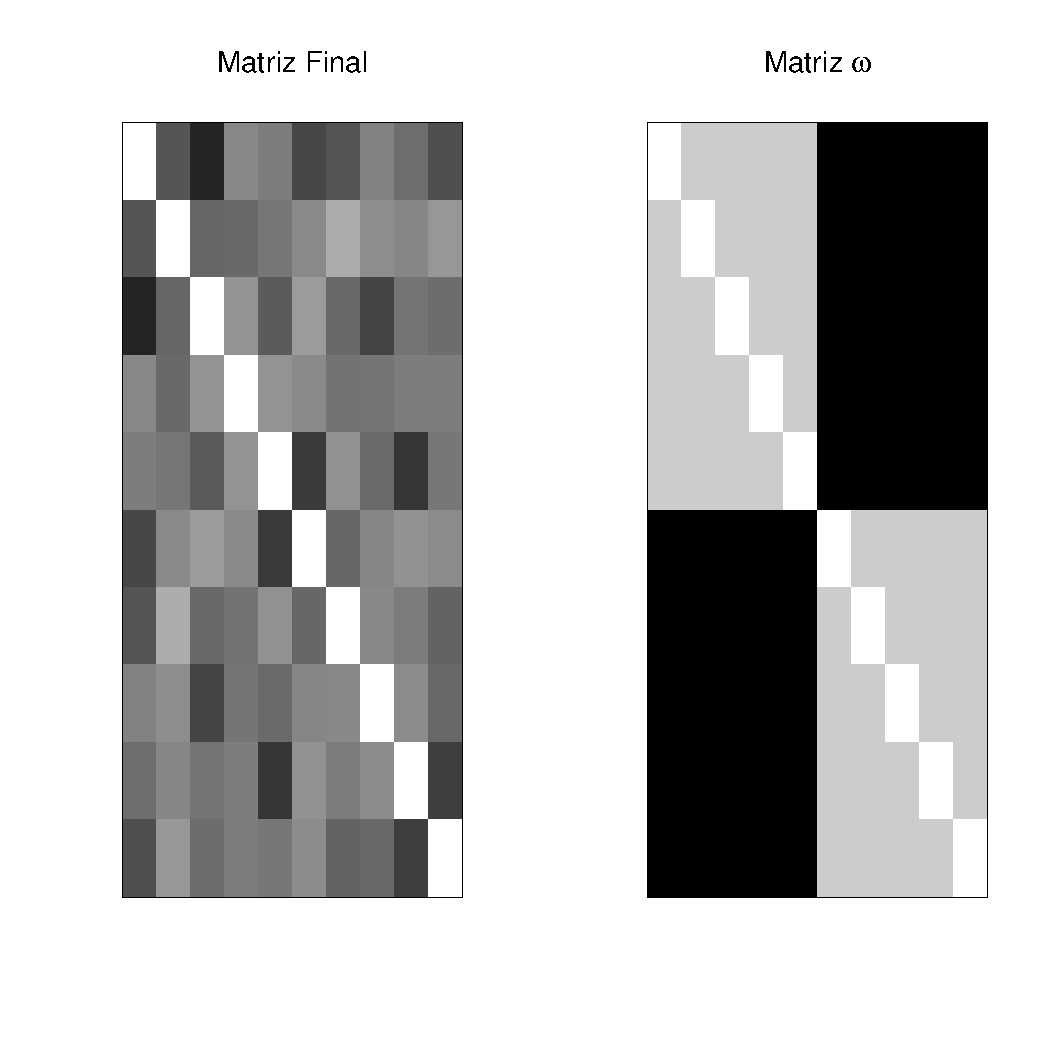
\includegraphics[width=150mm, height=80mm]{figuras/Mat10tracosDirecional}
   \caption{Comparação entre a matriz de correlação final para 10 traços
   após 10000 gerações de seleção direcional e estabilizadora
   representadas na figura \ref{jones10tracosDirecional} com a matriz
   $\omega$ da superfície de seleção.}
  \label{MatJones10tracosDirecional}
\end{figure}
\end{center}

Acreditamos que essa dificuldade em reproduzir os resultados encontrados
em sistemas com 2 e 3 traços no sistema com 10 traços se deve ao aumento
considerável do espaço possível de variação que a inclusão de cada novo
traço representa. 
O morfo-espaço cresce rapidamente com a inclusão de cada novo traço, e
as possibilidades para a matriz $M$ também. 
A seleção indireta então se torna muito fraca para promover o
alinhamento entre as matrizes, e a mutação não explora de forma adequada
o espaço da matriz mutacional, levando a uma situação de não alinhamento
mesmo com uma pressão seletiva considerável. 

\section{Resultados e Discussão $\cdot$ Matriz $B$}

Todas as simulações dessa seção começam com o mesmo estado inicial, com
a matriz $B$ totalmente formada por $1$, ou seja, integração total, e
todos os valores aditivos $0$, ou seja, todos os traços nulos. 
As primeiras gerações são dependentes desses estado inicial e não trazem
informação. Após cerca de $1000$ gerações o sistema já se encontra em
equilibrio seleção-mutação-deriva e pode ser analizado independentemente
do estado inicial.
Isso se reflete em todos gráficos como um transiente instável, seguido
de estabilidade dependente principalmente do tamanho populacional.
Discutimos esses efeitos e outros na próxima seção.

\subsection{Seleção Estabilizadora}

No segundo tipo de modelagem, começamos já com 10 traços sofrendo
seleção estabilizadora correlacionada dada pela matriz apresentada na
equação \ref{matw}. 
Exploramos então a influência de várias razões entre a taxa de mutação
nos alelos aditivos ($\mu$) e a taxa de mutação nas caselas da matriz
$B$ ($\mu_B$). 
Essa razão $\mu/\mu_B$ define como será a dinâmica temporal de mudança
entre dois níveis: o dos efeitos aditivos e o da atribuição desses
efeitos aos traços quantitativos. 
Conforme vemos nas figuras \ref{MatBEstab} e \ref{EstabRMuStats}, apesar de mudanças na
magnitude das correlações com o aumento da razão $\mu/\mu_B$, não
observamos o surgimento de módulos variacionais apenas com seleção
estabilizadora correlacionada. 

\begin{center}
\begin{figure}[htbp]
  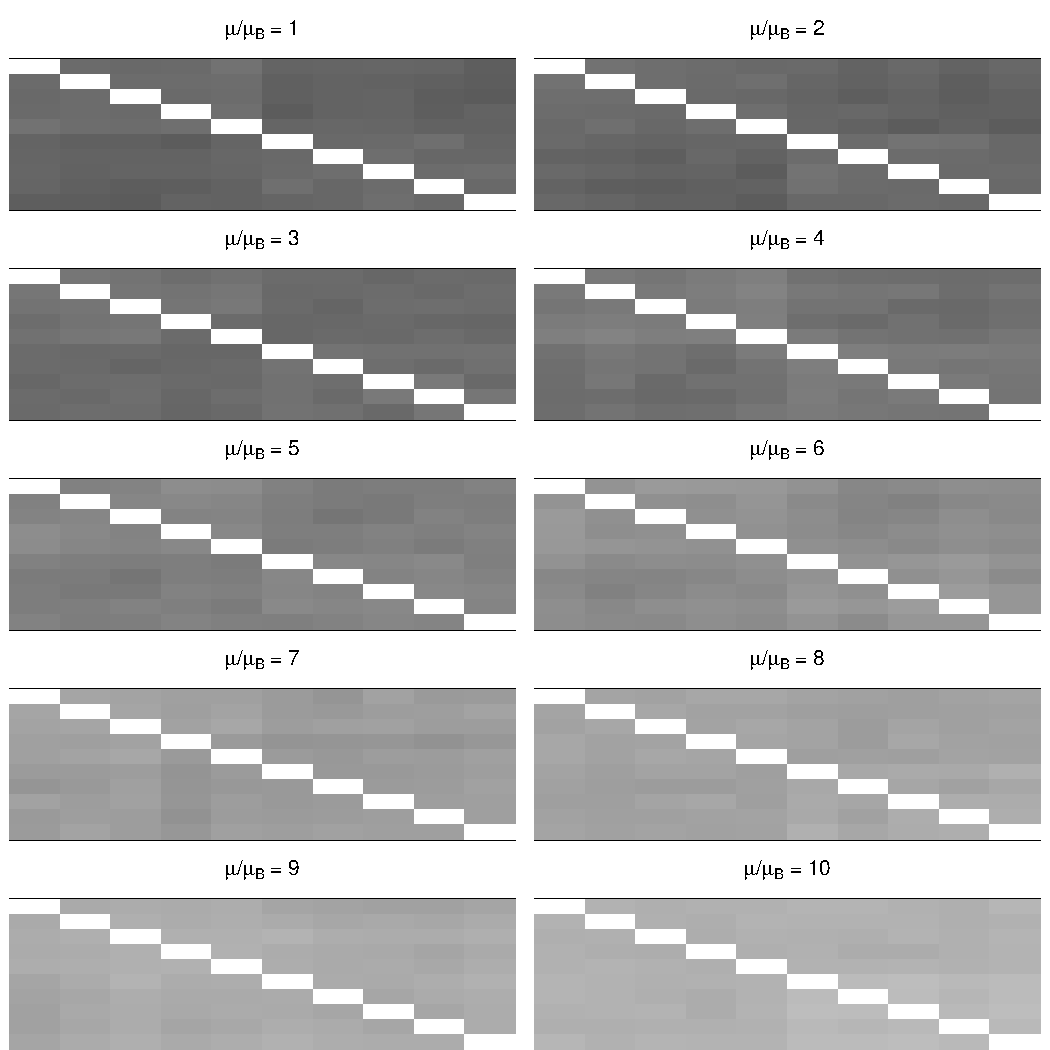
\includegraphics[width=150mm, height=180mm]{figuras/MatBEstabRMu}
   \caption{Matriz final média de 10 corridas para diferentes razões de
   $\mu$ e $\mu_B$, com seleção estabilizadora correlacionada com 2
   módulos.}
  \label{MatBEstab}
\end{figure}
\end{center}

\begin{center}
   \begin{figure}[htbp]
      \centering
      \subfloat [$\mu/\mu_B = 1$]{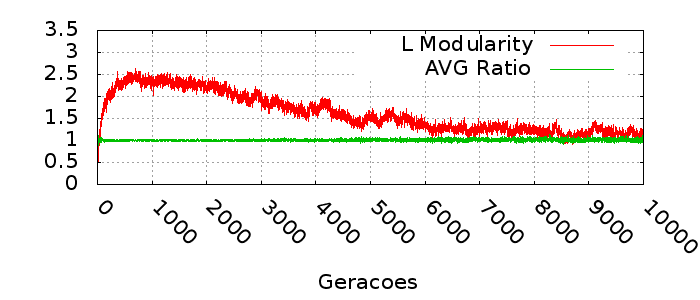
\includegraphics[width=70mm, height=30mm]{figuras/EstabRMuStats1.png}}\vspace{11pt}
      \subfloat [$\mu/\mu_B = 2$]{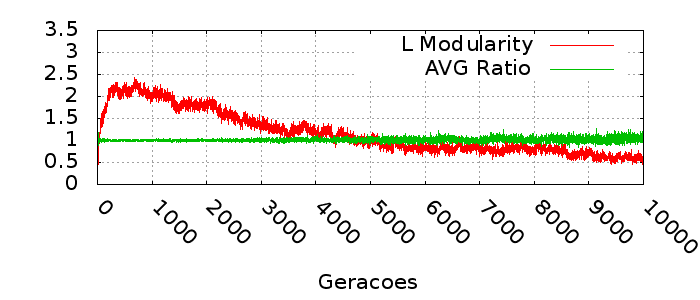
\includegraphics[width=70mm, height=30mm]{figuras/EstabRMuStats2.png}}\\ 
      \vspace{-18pt}
      \subfloat [$\mu/\mu_B = 3$]{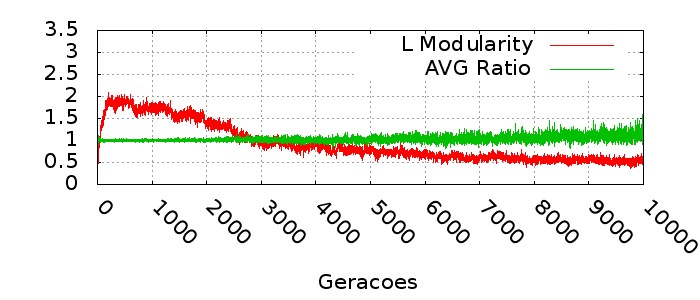
\includegraphics[width=70mm, height=30mm]{figuras/EstabRMuStats3.png}}\vspace{11pt} 
      \subfloat [$\mu/\mu_B = 4$]{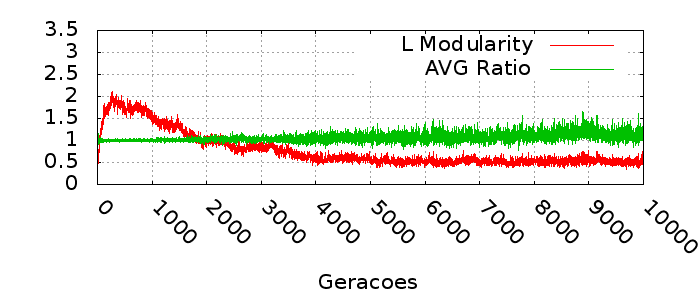
\includegraphics[width=70mm, height=30mm]{figuras/EstabRMuStats4.png}}\\
      \vspace{-18pt}
      \subfloat [$\mu/\mu_B = 5$]{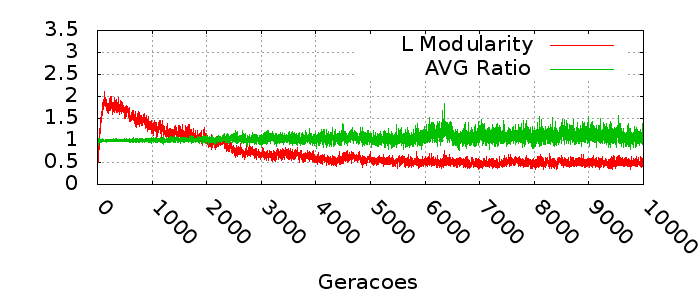
\includegraphics[width=70mm, height=30mm]{figuras/EstabRMuStats5.png}}\vspace{11pt}
      \subfloat [$\mu/\mu_B = 6$]{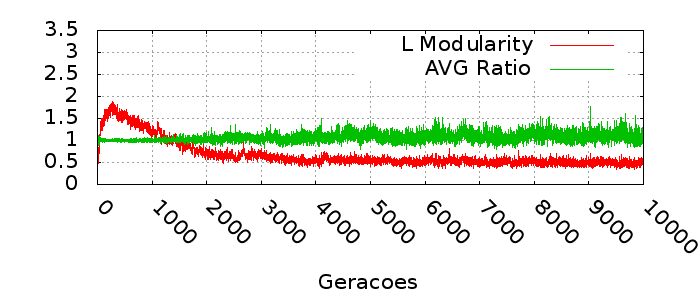
\includegraphics[width=70mm, height=30mm]{figuras/EstabRMuStats6.png}}\\
      \vspace{-18pt}
      \subfloat [$\mu/\mu_B = 7$]{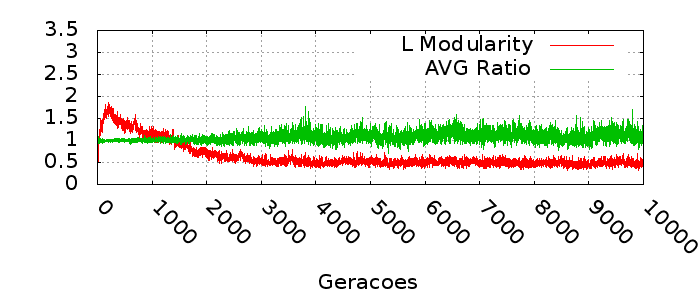
\includegraphics[width=70mm, height=30mm]{figuras/EstabRMuStats7.png}}\vspace{11pt}
      \subfloat [$\mu/\mu_B = 8$]{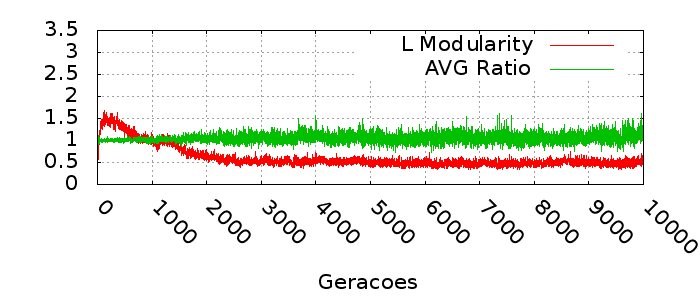
\includegraphics[width=70mm, height=30mm]{figuras/EstabRMuStats8.png}}\\
      \vspace{-18pt}
      \subfloat [$\mu/\mu_B = 9$]{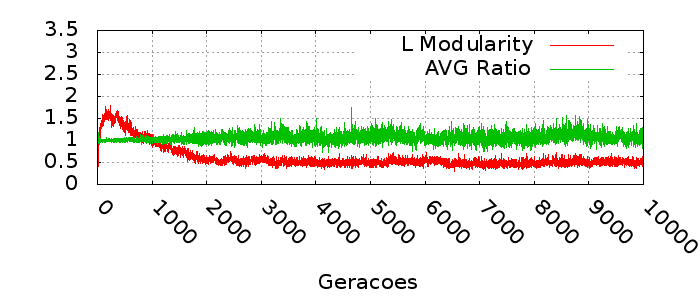
\includegraphics[width=70mm, height=30mm]{figuras/EstabRMuStats9.png}}\vspace{11pt}
      \subfloat [$\mu/\mu_B = 10$]{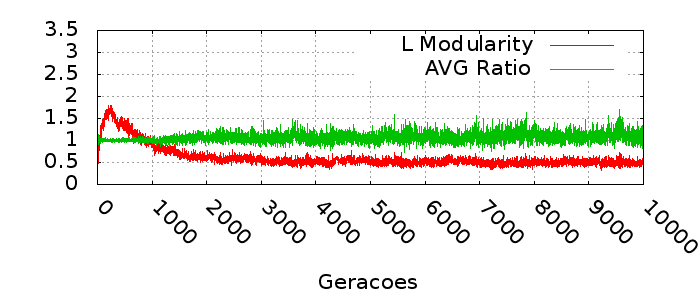
\includegraphics[width=70mm, height=30mm]{figuras/EstabRMuStats10.png}}\\
      \caption{Evolução típica de AVG-Ratio e modularidade $L$ para diferentes razões de
      $\mu$ e $\mu_B$, com seleção estabilizadora correlacionada com 2 módulos.}
      \label{EstabRMuStats}
   \end{figure}
\end{center}


\subsection{Seleção Direcional}

Com a inclusão de seleção direcional, como na figura
\ref{MatJones10tracosDirecional}, e $\mu/\mu_B = 0.1$, ainda não
observamos a formação de módulos na matriz G (figura \ref{RMu01}). 

\begin{center}
\begin{figure}[htbp]
  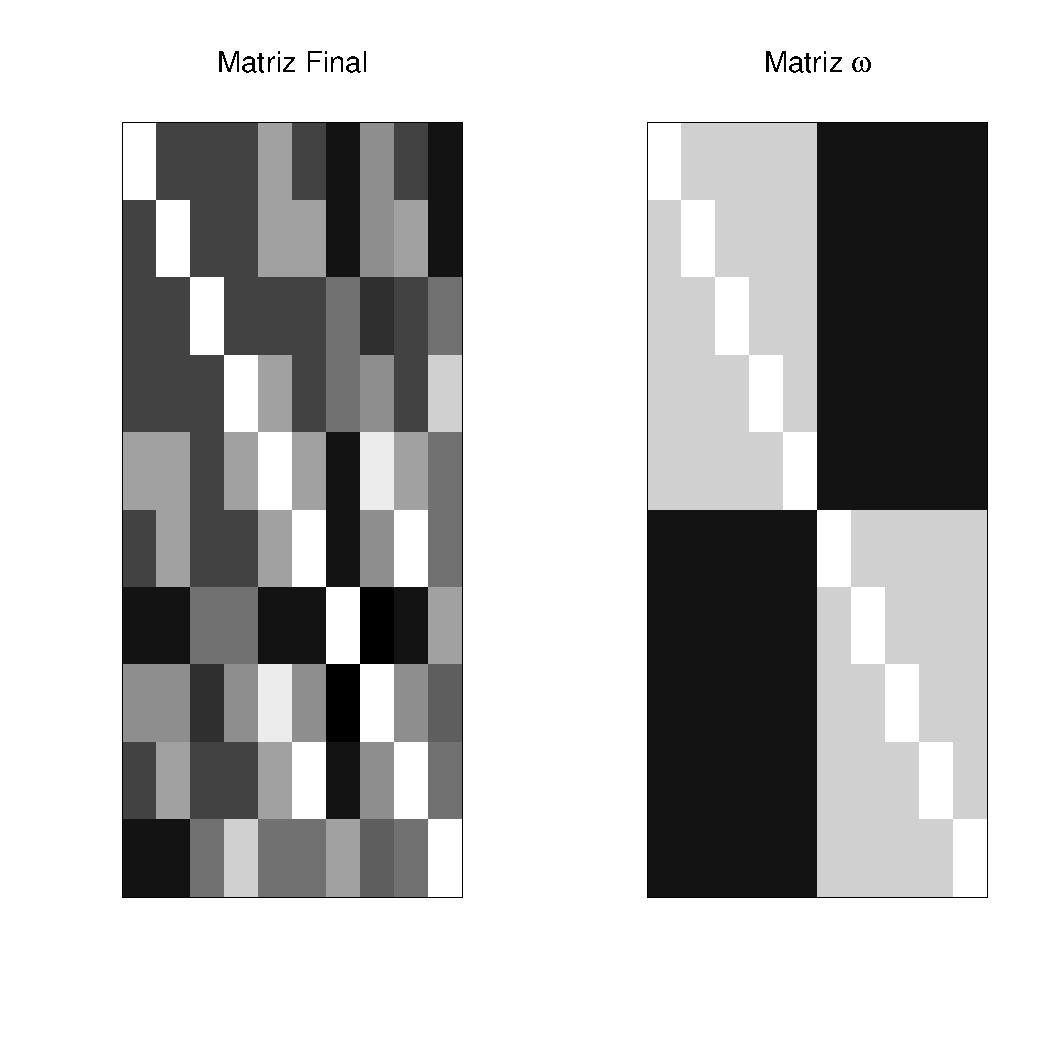
\includegraphics[width=150mm, height=80mm]{figuras/RMu01Omega}
   \caption{Comparação entre a matriz de correlação final média de 10
   corridas para o 10 traços após 10000
   gerações de seleção direcional e estbilizadora com a matriz $\omega$ da superfície de seleção e $\frac{\mu}{\mu_B}=0.1$, $Ne=2500$, $\Delta_S=0.2$, $m/p=2$}
  \label{RMu01}
\end{figure}
\end{center}

Porém, como vemos na figura \ref{MatBDirecional-RMu}, o aumento  na
razão $\mu/\mu_B$ aliada à seleção direcional é capaz de alterar essa
situação. 
Esse aumento parece promover um sistema capaz de responder de forma
eficiente às pressões seletivas impostas e gerar uma matriz G com a
estrutura modular privilegiada pela seleção estabilizadora e direcional. 
Lembramos que na ausência de seleção direcional esse efeito não é
observado, mesmo com as mesmas razões $\mu/\mu_B$. 
Na figura \ref{DirecionalRMuStats} vemos que razões baixas de $\mu/\mu_B$ levam
a sistemas bastante instáveis, apesar de modulares.
Para $\mu/\mu_B=1$, ou seja, com a taxa de mutação igual nos níveis
aditivo e ontogenético, o valor de AVG-Ratio flutua violentamente entre
as gerações, sugerindo uma modularidade muito instável.
A partir de $\mu/\mu_B=4$ o sistema se torna muito mais estável e
progressivamente menos modular.
Nós optamos por utilizar o valor $\mu/\mu_B=5$ nas simulações
subsequentes.
Essa opção se deu por uma série de fatores: nesse valor o sistema ainda
apresenta um aumento de modularidade ao longo das gerações; os valores
de modularidade $L$ e AVG-Ratio são bastante concordantes, sugerindo que
os módulos favorecidos pela seleção estão efetivamente sendo expressos
na população; e, por último, o sistema possui uma estabilidade razoável
sem se tornar estático.

Na figura \ref{MatBDirecionalNe2500RMu5} vemos um exemplo de corrida com
$N_e = 2500$ e $\mu/\mu_B=5$, mostrando claramente a separação de grupos
de correlação dentro de e entre módulos. 
Posteriormente, vamos explorar a influência do tamanho populacional na
estabilidade das matrizes geradas pelas nossas simulações (figura
\ref{posselecao}). 

\begin{center}
\begin{figure}[htbp]
  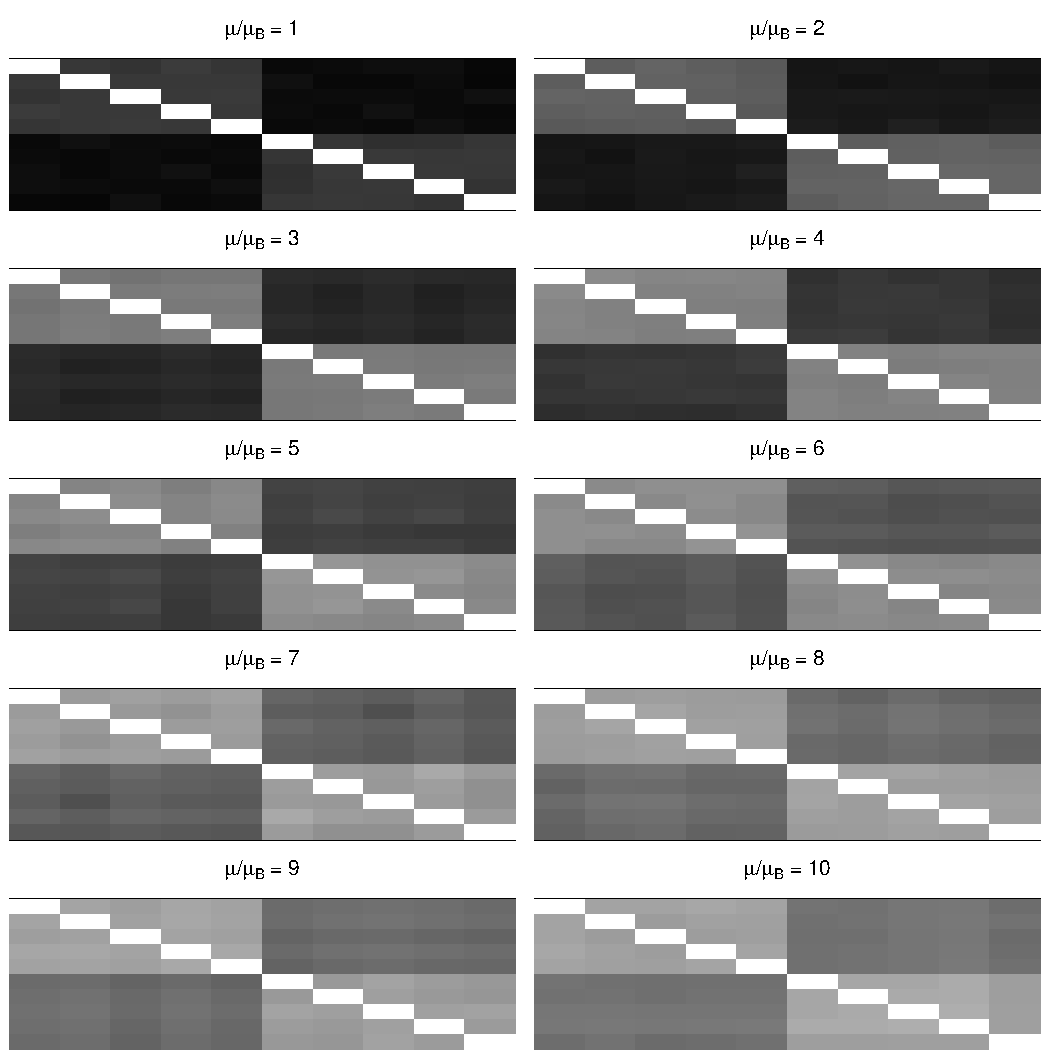
\includegraphics[width=150mm, height=180mm]{figuras/MatBDirecRMu}
   \caption{Matriz final média de 10 corridas para diferentes razões de
   $\frac{\mu}{\mu_B}$, com seleção estabilizadora correlacionada com 2
   módulos e seleção direcional correlacionada favorecendo os mesmos
   módulos. ($N_e=2500$, $\Delta_S=0.2$, $m/n=2$)}
  \label{MatBDirecional-RMu}
\end{figure}
\end{center}

\begin{center}
   \begin{figure}[htbp]
      \centering
      \subfloat [$\mu/\mu_B = 1$]{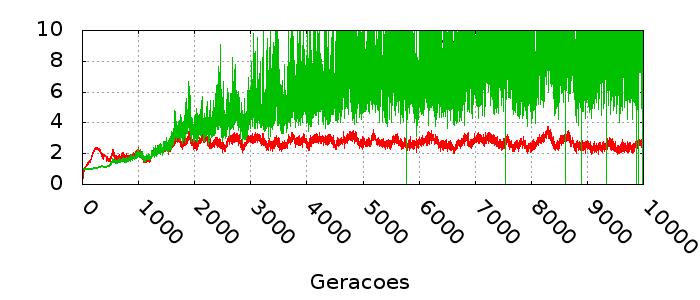
\includegraphics[width=70mm, height=30mm]{figuras/DirecionalRMuStats1.png}}\vspace{11pt}
      \subfloat [$\mu/\mu_B = 2$]{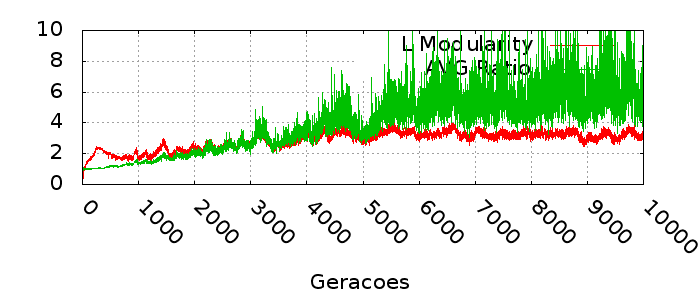
\includegraphics[width=70mm, height=30mm]{figuras/DirecionalRMuStats2.png}}\\ 
      \vspace{-18pt}
      \subfloat [$\mu/\mu_B = 3$]{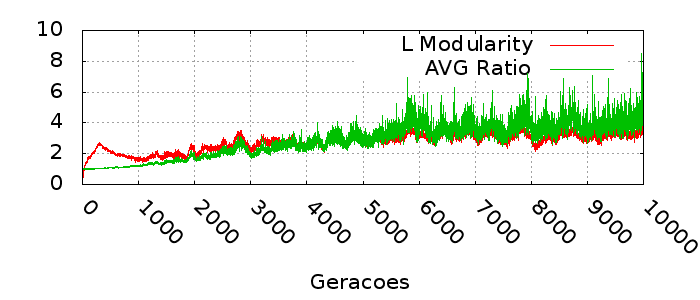
\includegraphics[width=70mm, height=30mm]{figuras/DirecionalRMuStats3.png}}\vspace{11pt} 
      \subfloat [$\mu/\mu_B = 4$]{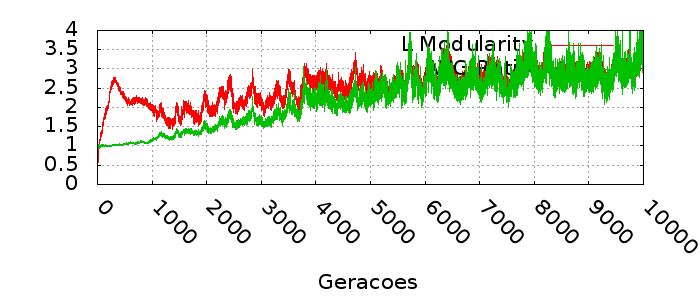
\includegraphics[width=70mm, height=30mm]{figuras/DirecionalRMuStats4.png}}\\
      \vspace{-18pt}
      \subfloat [$\mu/\mu_B = 5$]{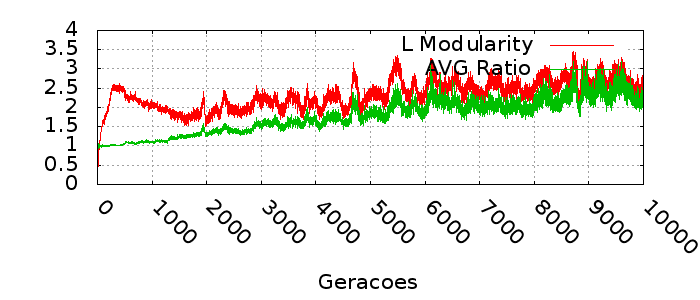
\includegraphics[width=70mm, height=30mm]{figuras/DirecionalRMuStats5.png}}\vspace{11pt}
      \subfloat [$\mu/\mu_B = 6$]{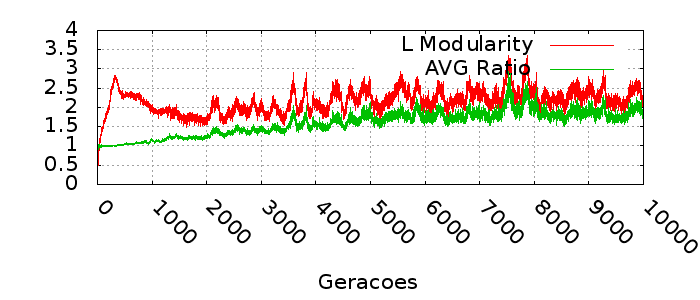
\includegraphics[width=70mm, height=30mm]{figuras/DirecionalRMuStats6.png}}\\
      \vspace{-18pt}
      \subfloat [$\mu/\mu_B = 7$]{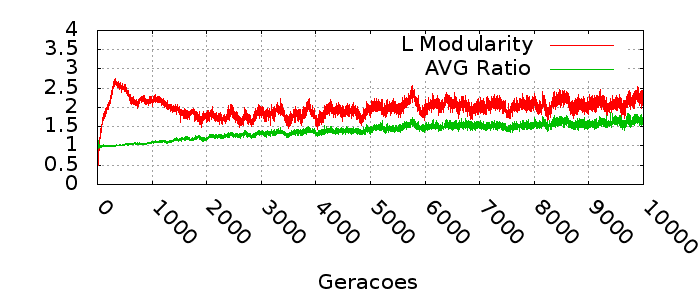
\includegraphics[width=70mm, height=30mm]{figuras/DirecionalRMuStats7.png}}\vspace{11pt}
      \subfloat [$\mu/\mu_B = 8$]{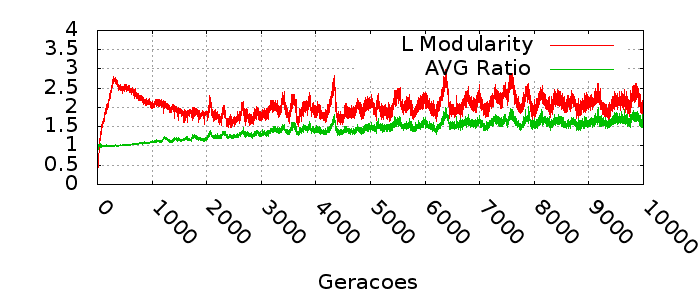
\includegraphics[width=70mm, height=30mm]{figuras/DirecionalRMuStats8.png}}\\
      \vspace{-18pt}
      \subfloat [$\mu/\mu_B = 9$]{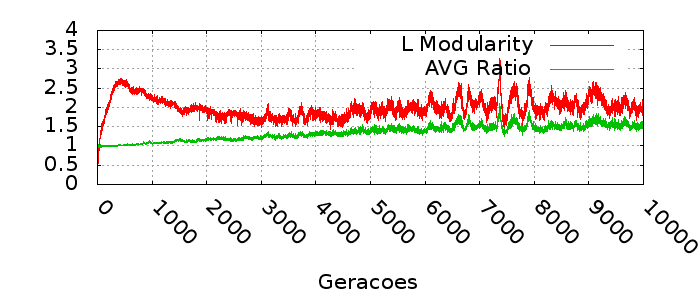
\includegraphics[width=70mm, height=30mm]{figuras/DirecionalRMuStats9.png}}\vspace{11pt}
      \subfloat [$\mu/\mu_B = 10$]{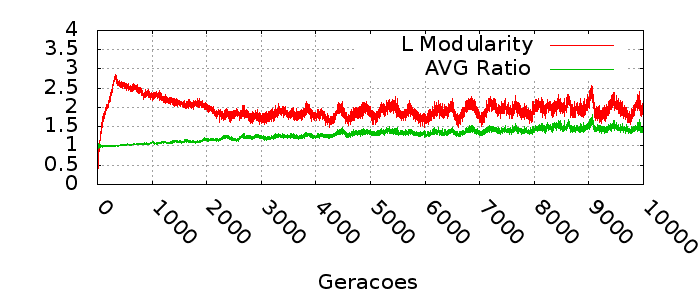
\includegraphics[width=70mm, height=30mm]{figuras/DirecionalRMuStats10.png}}\\
      \caption{Evolução típica de AVG-Ratio e modularidade $L$ para diferentes razões de
      $\mu$ e $\mu_B$, com seleção establizadora correlacionada com 2
      módulos e seleção direcional correlacionada favorecendo os mesmos
      módulos. Atenção para a mudança de escala nos eixos verticais. ($N_e=2500$, $\Delta_S=0.2$, $m/n=2$)}
      \label{DirecionalRMuStats}
   \end{figure}
\end{center}

\begin{center}
\begin{figure}[htbp]
  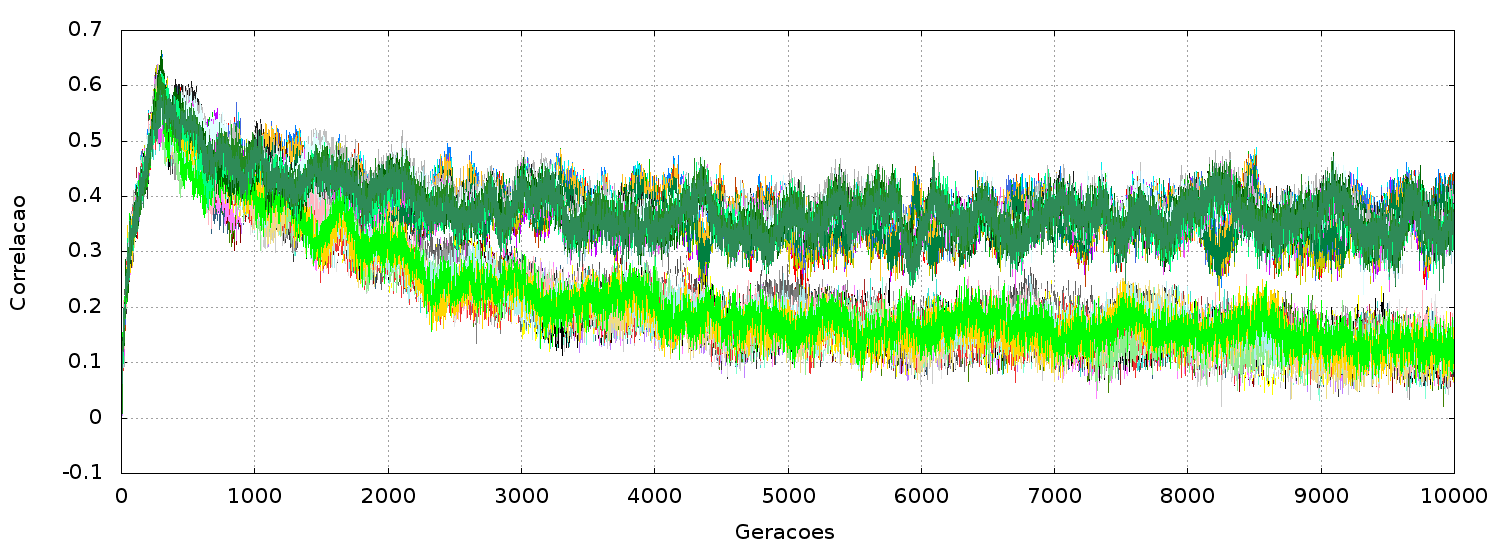
\includegraphics[width=150mm, height=55mm]{figuras/direcionalRMu5Ne2500IntSel200.png}
  \caption{Evolução da correlação entre dez traços ligados por efeitos
  pleiotrópicos controlados por uma função ontogenética linear binária
  variável, sofrendo seleção estabilizadora correlacionada
  e seleção direcional intensa para mudança correlacionada dentros dos
  módulos durante as 10000 gerações. 
  ($N_e = 2500$, $\mu/\mu_B=5$, $\Delta_S=0.2$, $m/p=2$)}
  \label{MatBDirecionalNe2500RMu5}
\end{figure}
\end{center}

Estamos interessados também na força de seleção direcional necessária
para gerar a estrutura modular nas matrizes de covariação. 
Nas figuras \ref{MatBIntSel110} e \ref{MatBIntSel1120} vemos matrizes
médias finais para 10 corridas com $N_e = 1000$, $\mu/\mu_B=5$ e
intensidade de seleção variável. 
Para isso, modificamos o quanto o pico adaptativo era alterado para cada
traço a cada geração, de $0.01$ até $0.2$ por geração durante 10000
gerações. 
Nas figuras \ref{IntSelStats10100} e \ref{IntSelStats110200} vemos
evoluções típicas de AVG-Ratio e modularidade $L$ para corridas com
várias intensidades de seleção, mostrando o quão estáveis e o quão
rápido os padrões modulares se estabelecem nessas condições.
Vemos que mesmo com um tamanho populacional considerável ($Ne = 2500$)
ainda observamos flutuções grandes.

A medida que aumentamos a intensidade de seleção os modulos se tornam
mais evidentes, mas acima de uma certa intensidade (delta $\simeq 0.06$)
esse efeito se torna mais discreto. 
Esse platô na resposta a seleção direcional pode ser explicado por como
funciona a nossa seleção. 
Quando a variância entre as aptidões na população for suficientemente
alta, apenas os indivíduos com maior aptidão vão se reproduzir, e,
dentro de limites\footnote{ Quando o pico se encotra suficientemente
longe da média da população, a variância nos valores de aptidão cai
novamente, pois todos os indivíduos tem aptidão próxima de zero, e a
chance de um indivíduo se reproduzir deixa de depender do fenótipo. 
Isso é uma limitação do esquema de seleção estritamente gaussiano.}, as
mudanças em $\Delta_S$ não alteram quais são esses indivíduos. 

\begin{center}
\begin{figure}[htbp]
  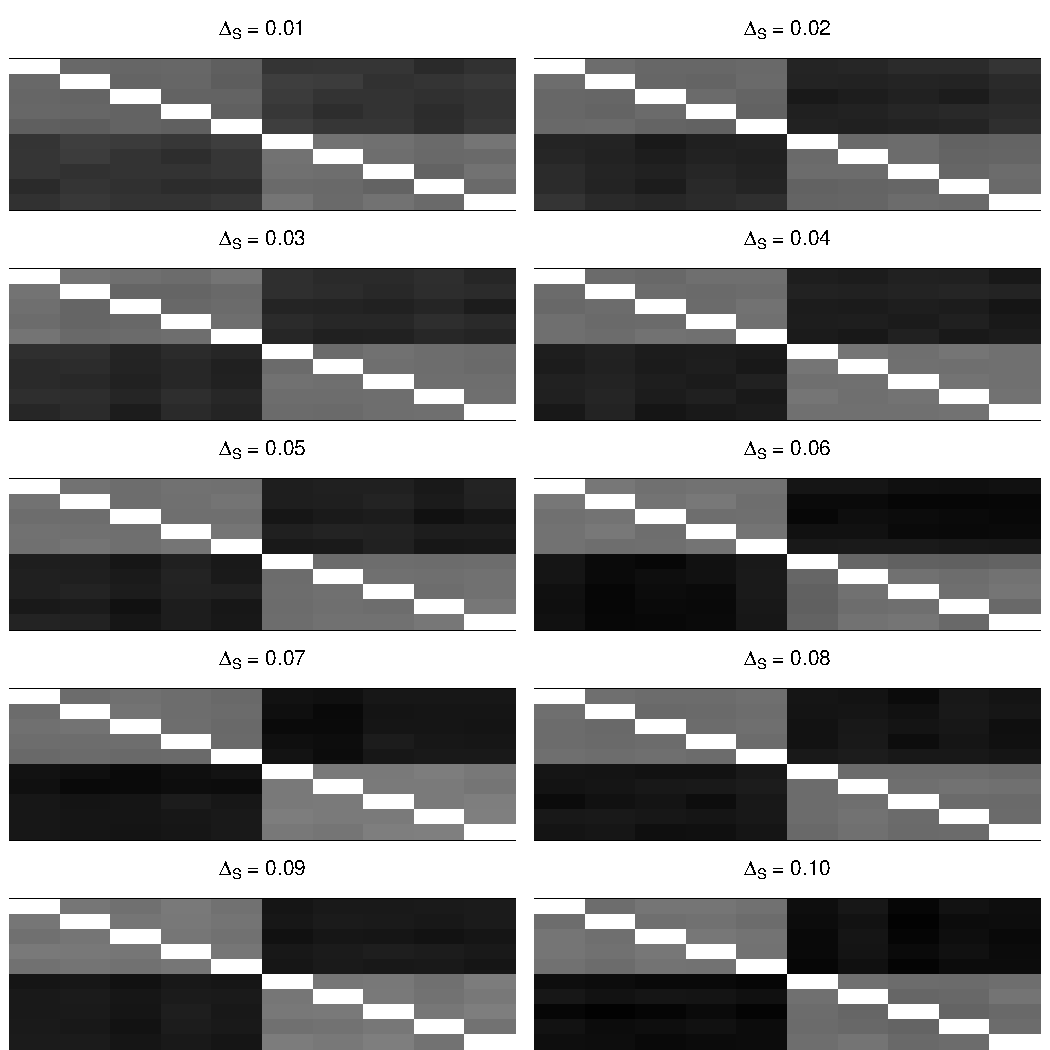
\includegraphics[width=150mm, height=180mm]{figuras/MatBDirecionalIntSel110}
   \caption{Matriz final média de 10 corridas com
   $\frac{\mu}{\mu_B} = 5$, $Ne = 1000$, $m/p=2$, sofrendo seleção estabilizadora correlacionada com 2
   módulos e seleção direcional com diferentes valores de $\Delta_S$.}
  \label{MatBIntSel110}
\end{figure}
\end{center}

\begin{center}
   \begin{figure}[htbp]
      \centering
      \subfloat [$\Delta_S = 0.01$]{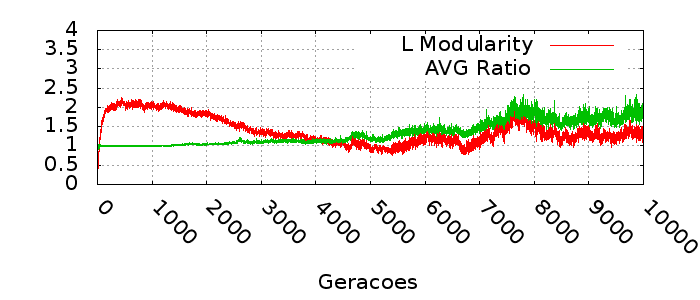
\includegraphics[width=70mm, height=30mm]{figuras/IntSelStats10.png}}\vspace{11pt}
      \subfloat [$\Delta_S = 0.02$]{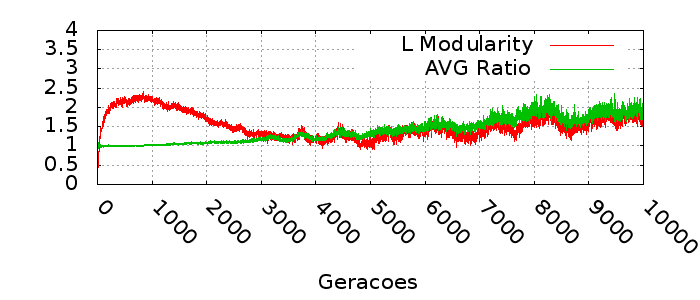
\includegraphics[width=70mm, height=30mm]{figuras/IntSelStats20.png}}\\ 
      \vspace{-18pt}
      \subfloat [$\Delta_S = 0.03$]{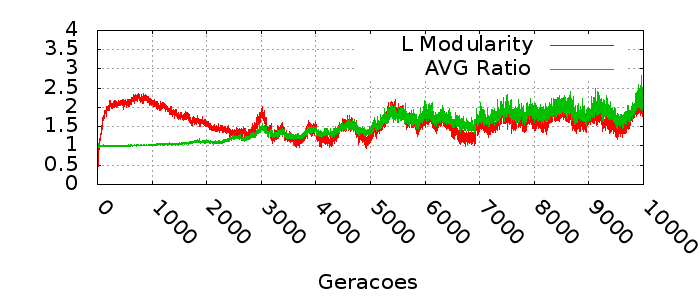
\includegraphics[width=70mm, height=30mm]{figuras/IntSelStats30.png}}\vspace{11pt} 
      \subfloat [$\Delta_S = 0.04$]{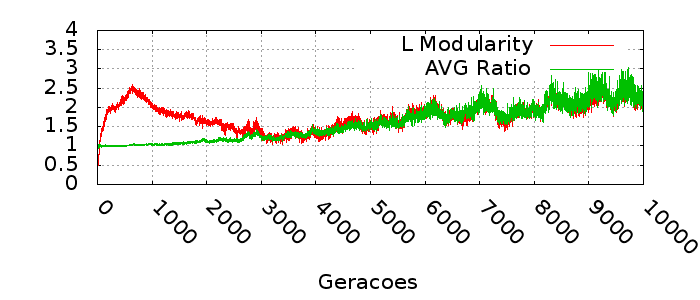
\includegraphics[width=70mm, height=30mm]{figuras/IntSelStats40.png}}\\
      \vspace{-18pt}
      \subfloat [$\Delta_S = 0.05$]{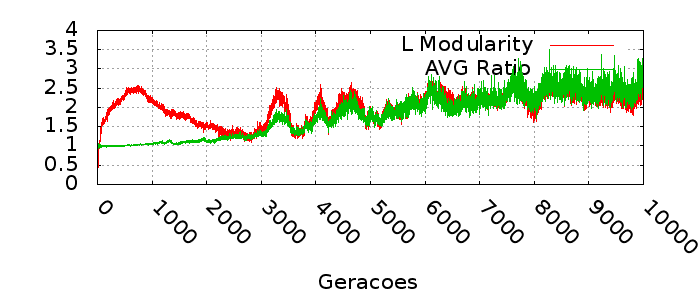
\includegraphics[width=70mm, height=30mm]{figuras/IntSelStats50.png}}\vspace{11pt}
      \subfloat [$\Delta_S = 0.06$]{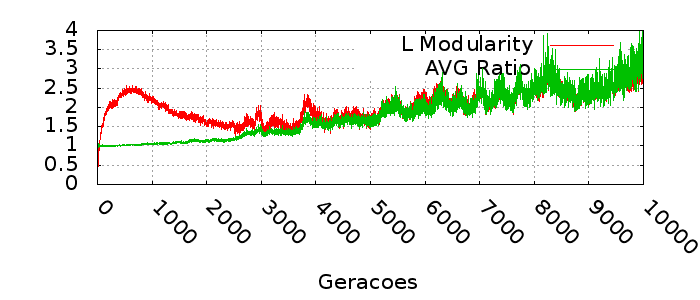
\includegraphics[width=70mm, height=30mm]{figuras/IntSelStats60.png}}\\
      \vspace{-18pt}
      \subfloat [$\Delta_S = 0.07$]{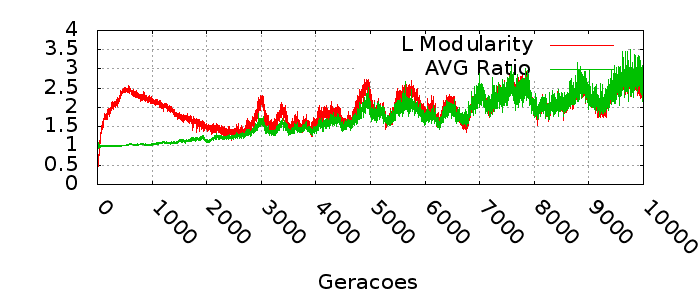
\includegraphics[width=70mm, height=30mm]{figuras/IntSelStats70.png}}\vspace{11pt}
      \subfloat [$\Delta_S = 0.08$]{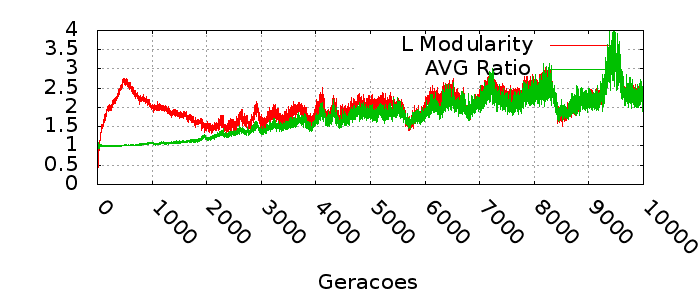
\includegraphics[width=70mm, height=30mm]{figuras/IntSelStats80.png}}\\
      \vspace{-18pt}
      \subfloat [$\Delta_S = 0.09$]{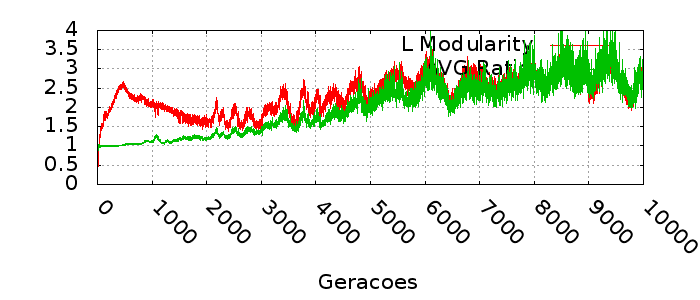
\includegraphics[width=70mm, height=30mm]{figuras/IntSelStats90.png}}\vspace{11pt}
      \subfloat [$\Delta_S = 0.1$]{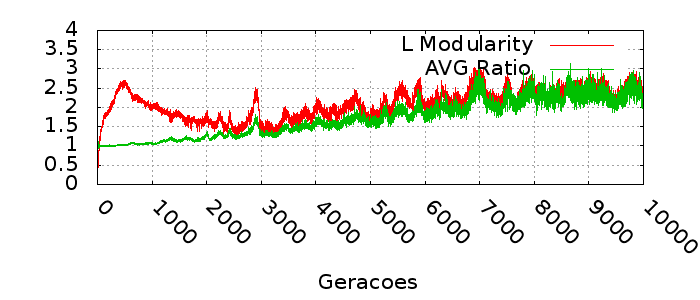
\includegraphics[width=70mm, height=30mm]{figuras/IntSelStats100.png}}\\
      \caption{ AVG-Ratio e modularidade $L$ para corridas com
         $\frac{\mu}{\mu_B} = 5$, $Ne = 2500$, $m/p=2$, sofrendo seleção
         estabilizadora correlacionada com 2 módulos e seleção direcional com
         diferentes valores de $\Delta_S$.}
      \label{IntSelStats10100}
   \end{figure}
\end{center}

\begin{center}
\begin{figure}[htbp]
  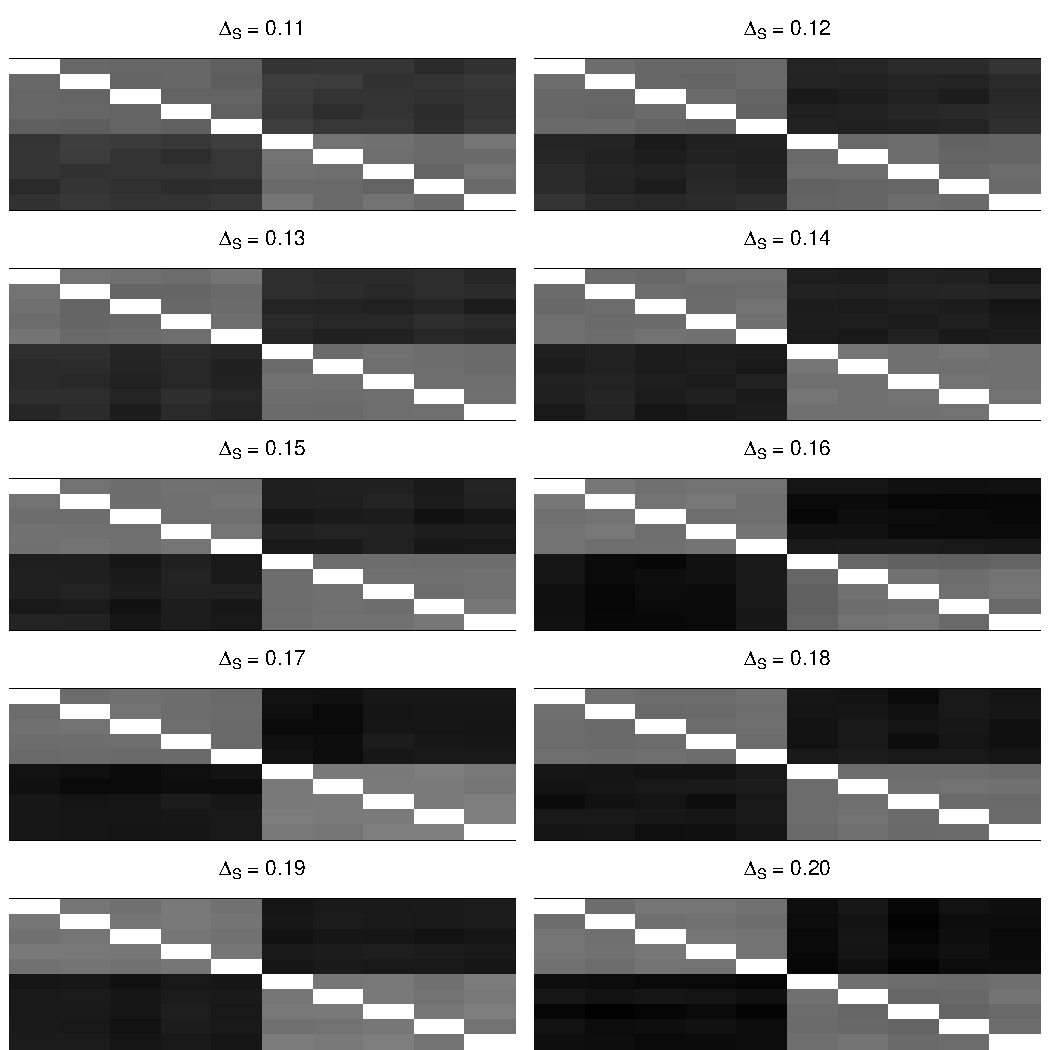
\includegraphics[width=150mm, height=180mm]{figuras/MatBDirecionalIntSel1120}
   \caption{Matriz final média de 10 corridas com
   $\frac{\mu}{\mu_B} = 5$, $Ne = 1000$, $m/p=2$, sofrendo seleção estabilizadora correlacionada com 2
   módulos e seleção direcional com diferentes valores de $\Delta_S$.}
  \label{MatBIntSel1120}
\end{figure}
\end{center}

\begin{center}
   \begin{figure}[htbp]
      \centering
      \subfloat [$\Delta_S = 0.11$]{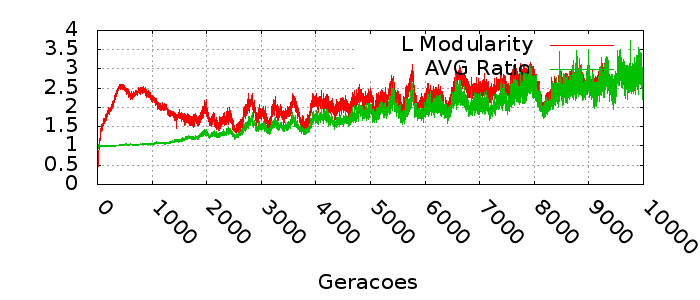
\includegraphics[width=70mm, height=30mm]{figuras/IntSelStats110.png}}\vspace{11pt}
      \subfloat [$\Delta_S = 0.12$]{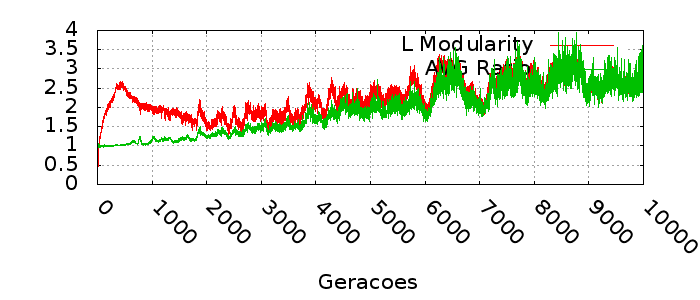
\includegraphics[width=70mm, height=30mm]{figuras/IntSelStats120.png}}\\ 
      \vspace{-18pt}
      \subfloat [$\Delta_S = 0.13$]{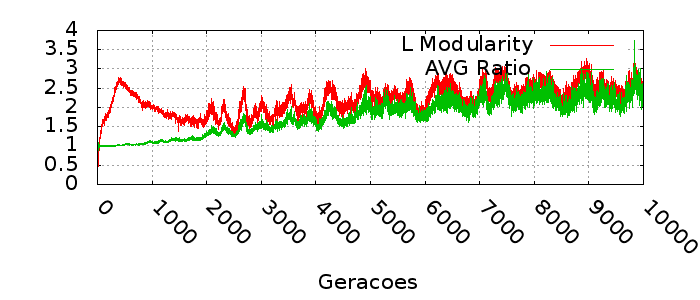
\includegraphics[width=70mm, height=30mm]{figuras/IntSelStats130.png}}\vspace{11pt} 
      \subfloat [$\Delta_S = 0.14$]{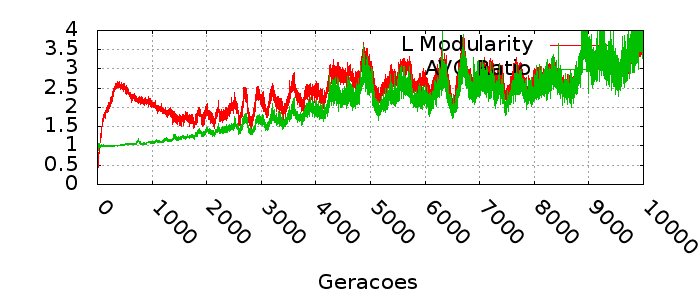
\includegraphics[width=70mm, height=30mm]{figuras/IntSelStats140.png}}\\
      \vspace{-18pt}
      \subfloat [$\Delta_S = 0.15$]{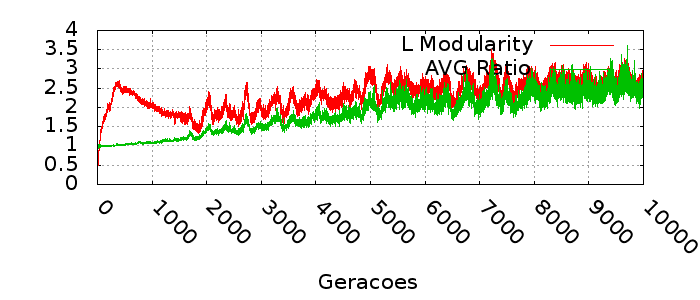
\includegraphics[width=70mm, height=30mm]{figuras/IntSelStats150.png}}\vspace{11pt}
      \subfloat [$\Delta_S = 0.16$]{\includegraphics[width=70mm, height=30mm]{figuras/IntSelStats160.png}}\\
      \vspace{-18pt}
      \subfloat [$\Delta_S = 0.17$]{\includegraphics[width=70mm, height=30mm]{figuras/IntSelStats170.png}}\vspace{11pt}
      \subfloat [$\Delta_S = 0.18$]{\includegraphics[width=70mm, height=30mm]{figuras/IntSelStats180.png}}\\
      \vspace{-18pt}
      \subfloat [$\Delta_S = 0.19$]{\includegraphics[width=70mm, height=30mm]{figuras/IntSelStats190.png}}\vspace{11pt}
      \subfloat [$\Delta_S = 0.2$]{\includegraphics[width=70mm, height=30mm]{figuras/IntSelStats200.png}}\\
      \caption{ AVG-Ratio e modularidade $L$ para corridas com
         $\frac{\mu}{\mu_B} = 5$, $Ne = 2500$, $m/p=2$, sofrendo seleção
         estabilizadora correlacionada com 2 módulos e seleção direcional com
         diferentes valores de $\Delta_S$.}
      \label{IntSelStats110200}
   \end{figure}
\end{center}

Outra questão relevante é o quão estáveis são os padrões de covariação
modulares gerados pela seleção direcional e estabilizadora. 
Para responder a essa pergunta nós sujeitamos populações de tamanhos
diferentes a uma mesma pressão seletiva intensa durante 5000 gerações
(periodo suficiente para o surgimento de módulos), seguidas de 5000
gerações de seleção estabilizadora correlacionada. 
Apesar da diferença entre as correlações dentro e entre modulos
diminuir, ainda observamos uma distinção estável entre elas (figura
\ref{posselecao}). 
O efeito do tamanho populacional é especialmente marcante nessas
condições, com populações grandes se mostrando mais eficientes na
manutenção prolongada dos padrões estabelecidos pela seleção direcional
(figuras \ref{posselecao} e \ref{posselecaoStats}). 

\begin{center}
\begin{figure}[htbp]
  \centering
  \subfloat [$Ne = 250$]{\includegraphics[width=70mm, height=50mm]{figuras/posselecao250.png}}\vspace{11pt}
  \subfloat [$Ne = 500$]{\includegraphics[width=70mm, height=50mm]{figuras/posselecao500.png}}\\
  \vspace{-18pt}
  \subfloat [$Ne = 1000$]{\includegraphics[width=70mm, height=50mm]{figuras/posselecao1000.png}}\vspace{11pt}
  \subfloat [$Ne = 2500$]{\includegraphics[width=70mm, height=50mm]{figuras/posselecao2500.png}}\\
  \vspace{-18pt}
  \subfloat [$Ne = 5000$]{\includegraphics[width=70mm, height=50mm]{figuras/posselecao5000.png}}\vspace{11pt}
  \subfloat [$Ne = 10000$]{\includegraphics[width=70mm, height=50mm]{figuras/posselecao10000.png}}\\
  \caption{Evolução da correlação entre dez traços ligados por efeitos
  pleiotrópicos controlados por uma matriz $B$ variável, sofrendo seleção estabilizadora correlacionada e seleção
  direcional para mudança correlacionada dentros dos módulos
  durante as 5000 primeiras gerações, seguidos de 5000 gerações de
  seleção estabilizadora correlacionada ($\Delta_S = 0.2$, $\mu/\mu_B=5$, $m/p=2$).}
  \label{posselecao}
\end{figure}
\end{center}

\begin{center}
\begin{figure}[htbp]
  \centering
  \subfloat [$Ne = 250$]{\includegraphics[width=70mm, height=50mm]{figuras/PosSelStatsNe250.png}}\vspace{11pt}
  \subfloat [$Ne = 500$]{\includegraphics[width=70mm, height=50mm]{figuras/PosSelStatsNe500.png}}\\
  \vspace{-18pt}
  \subfloat [$Ne = 1000$]{\includegraphics[width=70mm, height=50mm]{figuras/PosSelStatsNe1000.png}}\vspace{11pt}
  \subfloat [$Ne = 2500$]{\includegraphics[width=70mm, height=50mm]{figuras/PosSelStatsNe2500.png}}\\
  \vspace{-18pt}
  \subfloat [$Ne = 5000$]{\includegraphics[width=70mm, height=50mm]{figuras/PosSelStatsNe5000.png}}\vspace{11pt}
  \subfloat [$Ne = 10000$]{\includegraphics[width=70mm, height=50mm]{figuras/PosSelStatsNe10000.png}}\\
  \caption{Evolução de modularidade $L$ e AVG-Ratio para as correlações
     apresentadas na figura \ref{posselecao} ($\Delta_S = 0.2$, $\mu/\mu_B=5$, $m/p=2$).}
  \label{posselecaoStats}
\end{figure}
\end{center}


\begin{center}
\begin{figure}[htbp]
  \subfloat [$Ne = 250$]{\includegraphics[width=70mm, height=50mm]{figuras/posselecaoSemEstab250.png}}\vspace{11pt}
  \subfloat [$Ne = 500$]{\includegraphics[width=70mm, height=50mm]{figuras/posselecaoSemEstab500.png}}\\
  \vspace{-18pt}
  \subfloat [$Ne = 1000$]{\includegraphics[width=70mm, height=50mm]{figuras/posselecaoSemEstab1000.png}}\vspace{11pt}
  \subfloat [$Ne = 2500$]{\includegraphics[width=70mm, height=50mm]{figuras/posselecaoSemEstab2500.png}}\\
  \vspace{-18pt}
  \subfloat [$Ne = 5000$]{\includegraphics[width=70mm, height=50mm]{figuras/posselecaoSemEstab5000.png}}\vspace{11pt}
  \subfloat [$Ne = 10000$]{\includegraphics[width=70mm, height=50mm]{figuras/posselecaoSemEstab10000.png}}\\
  \caption{Evolução da correlação entre dez traços ligados por efeitos
  pleiotrópicos controlados por uma matriz $B$ variável, sofrendo seleção estabilizadora correlacionada e seleção
  direcional para mudança correlacionada dentros dos módulos
  durante as 5000 primeiras gerações, seguidos de 5000 gerações de
  seleção estabilizadora não correlacionada ($\Delta_S = 0.2$, $\mu/\mu_B=5$, $m/p=2$).}
  \label{posselecaoSemEstab}
\end{figure}
\end{center}

\begin{center}
\begin{figure}[htbp]
  \centering
  \subfloat [$Ne = 250$]{\includegraphics[width=70mm, height=50mm]{figuras/SemEstabPosSelStatsNe250.png}}\vspace{11pt}
  \subfloat [$Ne = 500$]{\includegraphics[width=70mm, height=50mm]{figuras/SemEstabPosSelStatsNe500.png}}\\
  \vspace{-18pt}
  \subfloat [$Ne = 1000$]{\includegraphics[width=70mm, height=50mm]{figuras/SemEstabPosSelStatsNe1000.png}}\vspace{11pt}
  \subfloat [$Ne = 2500$]{\includegraphics[width=70mm, height=50mm]{figuras/SemEstabPosSelStatsNe2500.png}}\\
  \vspace{-18pt}
  \subfloat [$Ne = 5000$]{\includegraphics[width=70mm, height=50mm]{figuras/SemEstabPosSelStatsNe5000.png}}\vspace{11pt}
  \subfloat [$Ne = 10000$]{\includegraphics[width=70mm, height=50mm]{figuras/SemEstabPosSelStatsNe10000.png}}\\
  \caption{Evolução de modularidade $L$ e AVG-Ratio para as correlações
     apresentadas na figura \ref{posselecao} ($\Delta_S = 0.2$, $\mu/\mu_B=5$, $m/p=2$).}
  \label{posselecaoSemEstabStats}
\end{figure}
\end{center}

Ainda na questão da estabilidade dos padrões de covariação, o papel da
seleção estabilizadora correlacionada pode ser avaliado sujeitando as
populações à seleção direcional e estabilizadora correlacionada por 5000
gerações, seguidas de 5000 gerações de seleção estabilizadora não
correlacionada, apenas mantendo a média de cada traço individualmente.
Nas figura \ref{posselecaoSemEstab} e \ref{posselecaoSemEstabStats}
podemos ver a importância da seleção estabilizadora correlacionada na
manutenção dos padrões modulares gerados pela seleção direcional. 
Comparando cada tamanho populacional mostrado nas figuras
\ref{posselecao}, \ref{posselecaoStats} e \ref{posselecaoSemEstab},
\ref{posselecaoSemEstabStats} podemos ver uma degradação muito mais
acentuada dos padrões modulares na ausência da seleção
estabilizadora correlacionada. 

A importância da seleção estabilizadora para explicar padrões de estase
no registro fóssil foi amplamente discutida em \cite{Charlesworth1982a}.
No contexto de padrões de covariação, seleção estabilizadora
correlacionada também foi apontada como uma provável explicação para a
estabilidade de padrões de covariação observados na natureza
\citep{Cheverud1984, Marroig2001, Porto2008}. 
Nossos resultados dão credibilidade a essa hipótese. 
A origem dessa seleção estabilizadora pode ser atribuida a fatores
internos dos organismos, como restrições ontogenéticas responsáveis pela
coesão entre as partes do indivíduo. 
Como essas restrições estão sempre presentes, a seleção correlacionada
está sempre presente e os padrões tendem a se manter estáveis. 

Um parâmetro ainda não mencionado é o número de alelos $m$ envolvidos na
determinação do valor fenotípico de cada um dos $p$ traços. 
No nosso esquema de simulação, aumentar o valor da razão $m/p$ é análogo
a aumentar a força de recombinação, pois o valor de $m$ define o número
de unidades recombinantes segregando na população. 
Podemos pensar em $m$ como o número de cromossomos no genôma do
indivíduo, em vez de pensar nele como número de alelos individualmente. 
Até agora a razão $m/p$ foi mantida em 2, um valor suficiente para
promover respostas complexas de todos os traços mas ainda
computacionalmente viável. 
A figura \ref{MB} mostra como o aumento na razão $m/p$ afeta a evolução
das correlações fenotípicas nas populações sujeitas a seleção direcional
intensa e seleção estabilizadora correlacionada. 

\begin{center}
\begin{figure}[htbp]
   \centering
  \subfloat [$m/p = 2$]{\includegraphics[width=70mm, height=40mm]{figuras/MB20.png}}\vspace{11pt}
  \subfloat [$m/p = 3$]{\includegraphics[width=70mm, height=40mm]{figuras/MB30.png}}\\
  \vspace{-18pt}
  \subfloat [$m/p = 4$]{\includegraphics[width=70mm, height=40mm]{figuras/MB40.png}}\vspace{11pt}
  \subfloat [$m/p = 5$]{\includegraphics[width=70mm, height=40mm]{figuras/MB50.png}}\\
  \vspace{-18pt}
  \subfloat [$m/p = 6$]{\includegraphics[width=70mm, height=40mm]{figuras/MB60.png}}\vspace{11pt}
  \subfloat [$m/p = 7$]{\includegraphics[width=70mm, height=40mm]{figuras/MB70.png}}\\
  \vspace{-18pt}
  \subfloat [$m/p = 8$]{\includegraphics[width=70mm, height=40mm]{figuras/MB80.png}}\vspace{11pt}
  \subfloat [$m/p = 9$]{\includegraphics[width=70mm, height=40mm]{figuras/MB90.png}}\\
  \caption{Evolução da correlação entre dez traços ligados por efeitos
  pleiotrópicos controlados por uma função ontogenética linear binária
  variável sofrendo seleção estabilizadora correlacionada e seleção
  direcional intensa para mudança correlacionada dentros dos módulos,
  para diferentes valores do número de alelos. ($Ne=5000$, $\mu/\mu_B=5$, $\Delta_S=0.2$)}
  \label{MB}
\end{figure}
\end{center}

Vemos na figura \ref{MB} que o aumento do número de alelos torna o
sistema mais lento em adquirir um caráter modular. 
Isso pode ser associado com o aumento na recombinação, que age na
direção oposta a das forças seletivas direcionais e estabilizadora
correlacionada. 
Isso nos levou a crer que tempos mais longos de seleção poderiam gerar o
mesmo resultado que o obtido com valores baixos de $m/p$. 
Na figura \ref{MBLR} vemos duas corridas longas, de 20000 gerações, com
$m/p = 9$ e $10$, mostrando o tempo de estabilização mais longo e a
modularidade mais discreta, com menor diferença nas correlações dentro
de e entre módulos. 
Isso pode ser associado à força de recombinação aumentada. 

\begin{center}
\begin{figure}[htbp]
  \centering
  \subfloat [$m/p = 9$]{\includegraphics[width=150mm, height=55mm]{figuras/MBLR90.png}}\vspace{11pt}
  \vspace{-18pt}
  \subfloat [$m/p = 10$]{\includegraphics[width=150mm, height=55mm]{figuras/MBLR100.png}}\vspace{11pt}
  \caption{Evolução da correlação entre dez traços ligados por efeitos
  pleiotrópicos controlados por uma função ontogenética linear binária
  variável sofrendo seleção estabilizadora correlacionada e seleção
  direcional intensa para mudança correlacionada dentros dos módulos,
  para diferentes valores do número de alelos. ($Ne=5000$, $\mu/\mu_B=5$, $\Delta_S=0.2$)}
  \label{MBLR}
\end{figure}
\end{center}
